%% content.tex
%%

%% ==============
\chapter{Experiment}
\label{ch:Experiment}
%% ==============

The knapsack problem introduced in Section \ref{ch:Literature Review:sec:Information Overload in a knapsack problem} is used to test the described hypotheses in our experiment. A \ac{GUI} is designed to provide an intuitive approach to participants. The experiment is conducted using the \ac{AMT} website and it reached 400 participants.

%% ===========================
\section{Knapsack Problem}
\label{ch:Experiment:sec:Knapsack}

The knapsack problem used in this thesis is the 0-1-knapsack problem. This problem maximizes the cumulated value of items under a given weight restriction.
\begin{equation}
\begin{split}
\max\limits_{x_j} \sum_{j=1}^{n} v_j x_j \quad
s.t. \sum_{j=1}^{n} w_j x_j \leq W \quad \\
x_j \in \{0,1\} \quad for \quad j = 1, \dots, n \\
v_j := \text{value of item j} \quad w_j := \text{weight of item j}
\end{split}
\end{equation}

Table \ref{tab:KnapsackParamters} shows the given parameters for the considered 0-1-knapsack problem. The width of the knapsack, or the pixel width, represents the given weight restriction for the problem. There are 100 items to choose from and the weight of each item ranges from 20 to 80 units, and the benefit is defined as a number between 0 and 80.
\begin{table}[h] % Parameters for Knapsack
  \centering
    \begin{tabular}{c|c}
    \textbf{Parameter} & \multicolumn{1}{c}{\textbf{Fixed value}} \bigstrut[b]\\
    \hline
    \textbf{W} & 694 \bigstrut\\
    \hline
    \textbf{n} & 100 \bigstrut\\
    \hline
    \textbf{$w_j$ range} & \multicolumn{1}{c}{[20,80]} \bigstrut\\
    \hline
    \textbf{$v_j$ range} & \multicolumn{1}{c}{[0,80]} \bigstrut\\
    \hline
    \end{tabular}%
  \caption{Fixed parameters for the knapsack problem}
    \label{tab:KnapsackParamters}
\end{table}%
\newpage
Since the knapsack problem is an NP-hard problem, individuals are faced with a high rate of complexity and are further challenged with finding a solution in reasonable time. A "greedy approach" is used to model a potential game strategy used by participants to tackle the optimization.
The optimal solution is calculated by a pseudo-polynomial time algorithm using dynamic programming.

%% ===========================

\paragraph{Greedy Algorithm}
The greedy approach can be split into two steps. First, the items are sorted according to the ratio of their benefit and weight in descending order. Second, the items are added to the knapsack as long as it is not full.\\

\begin{algorithm} % Greedy
\LinesNumbered
\setcounter{AlgoLine}{0}
\SetNoFillComment
 \SetAlgoLined
 \tcc{items:=all available items, W:= knapsack limit }
 \KwIn{W, items}
 \KwResult{\ac{GA} solution to knapsack problem }
Sort items according to the ratio in descending order\;

knapsackSize=0, knapsackValue=0\;

 \For{item in items}{
    \If{knapsackSize+item.weight $\leq$ W}{
  	 knapsackValue+= item.benefit\;
  	 
	 knapsackSize += item.weight\;
   }
 }
\Return knapsackValue\;

\caption{Greedy Algorithm}
\end{algorithm}

\paragraph{Dynamic Programming Algorithm}
\label{par:DynamicProgrammingAlgorithm}
Since the greedy approach does not guarantee to find the most efficient, optimal solution for the knapsack problem, a different approach is used to calculate the optimal solution. The \ac{DPA} introduced by \cite{Kleinberg2005}  divides the problem into sub problems and can be solved in O(nW) time with W being the maximum weight of the knapsack.
\begin{algorithm} % Dynamic Programming
\LinesNumbered
\setcounter{AlgoLine}{0}
\SetNoFillComment
 \SetAlgoLined
 \tcc{items:=all available items, W:= knapsack limit }
 \KwIn{W, items}
 \KwResult{\ac{DPA} solution to knapsack problem }
 
i = 100\;

R = Matrix (100 x 694), each element with value 0\;

 \For{item in items}{
 \For{j=0 to limit}{
\If{item.weight $\leq$ j}{
  	 R[i][j] = max(item.benefit+R[i+1][j-item.weight], R[i+1][j])
   }
 } i - -
 }
\Return R[i][limit]; 
\caption{Dynamic Programming Algorithm}
\end{algorithm}
\paragraph{Comparability of the problems' difficulty}
To ensure the value of the statistical analysis across treatments and rounds, the underlying knapsack problems are designed to be sufficiently similar. For this purpose, a benchmark is introduced to compare the difficulty of knapsack problems and to design equally difficult problems.

The \textit{benchmark} is computed as the relative difference between the computed solution by the \ac{DPA} and the \ac{GA}. The greater the benchmark, the harder the problem.
The setup algorithm runs 100 times to ensure a sufficiently high benchmark.
\begin{equation}
benchmark = \Big(\dfrac{\text{\ac{DPA} solution}}{\text{\ac{GA} solution}} -1\Big) * 100\%
\end{equation}

\subparagraph{Comparability across treatments and rounds}
Four different knapsack problems are created in our experiment, one for each round plus the Trial round. To ensure the \textbf{comparability across rounds}, the benchmark is used to identify hard problems. For each round, the benchmark is calculated and the values are checked to be sufficiently similar.
 
In order to compare the performance of participants in \textbf{different treatments}, the underlying knapsack problems are the same for each individual round.
 \begin{figure}[htp] % Colour Scheme Benefit
\begin{center}
  \includegraphics[height = 0.4\textwidth]{colourSchemeBenefit.pdf}
\caption{Colours assigned to benefit range}
\label{fig:colourSchemeBenefit}
\end{center}
\end{figure}
Consequently, the distribution of the benefits and weights of each box is the same, the only difference is the assignation of colours. In the 2-colour treatment, one colour covers a wide range of benefit values, whereas in the 15-colour setup, one colour represents a smaller range of colours (refer to Figure \ref{fig:colourSchemeBenefit}).  Consequently, there are two opposing trends when increasing the number of colours. The more colours there are, the more alternatives there are to choose from, so the complexity of the task might increase. In contrast to that, the range of the benefit within one colour gets smaller, so participants can better distinguish between different benefit values.

%% ===========================
\paragraph{Setup}
\label{ch:Experiment:sec:Setup}
%% ===========================

The setup of the game\footnote{For the algorithm, refer to Appendix \ref{Appendix-Algorithm}.} is prepared before uploading the game. 
Each treatment is assigned 4 rounds with 100 boxes per round. The first round is the Test round\footnote{No data was conducted from the Trial round.} while the other 3 rounds are shown during the actual game.
Each box is randomly\footnote{The used random function returns a randomly determined value in a given range. The return values are uniformly distributed (\href{http://hg.python.org/cpython/file/2.7/Lib/random.py}{Source code}).} assigned a weight in the range of 20 to 80 units. This value represents the width of the boxes in pixel in the game.



%% ===========================
\section{Interface}
\label{ch:Experiment:sec:Interface}
%% ===========================
The items the participant can choose from are modelled as boxes. The width of each box represents its weight; every box has the same height. Thus, the wider the box, the greater the weight. 
The colour of the box represents the benefit.

\paragraph{Colour scale}
The colour scale used for each treatment aims to provide an intuitive range of colours that are also easily distinguishable. A traffic light colour scale was first favoured  since it is a well-known and intuitive colour pattern. Trial runs, however, showed that participants had problems distinguishing the colours when they were dealing with 11 or 15 colours. Green boxes were especially hard to differentiate for test participants. Furthermore, a colour-blindness test would have been necessary to identify colour-blind users.
As a result, we use a grey scale as shown in Figure \ref{fig:colourScheme}. This colour scale is both intuitive and accessible to colour-blind users and the grey levels are easy to distinguish.\\
\begin{figure}[htp] % Colour Scheme
\begin{center}
  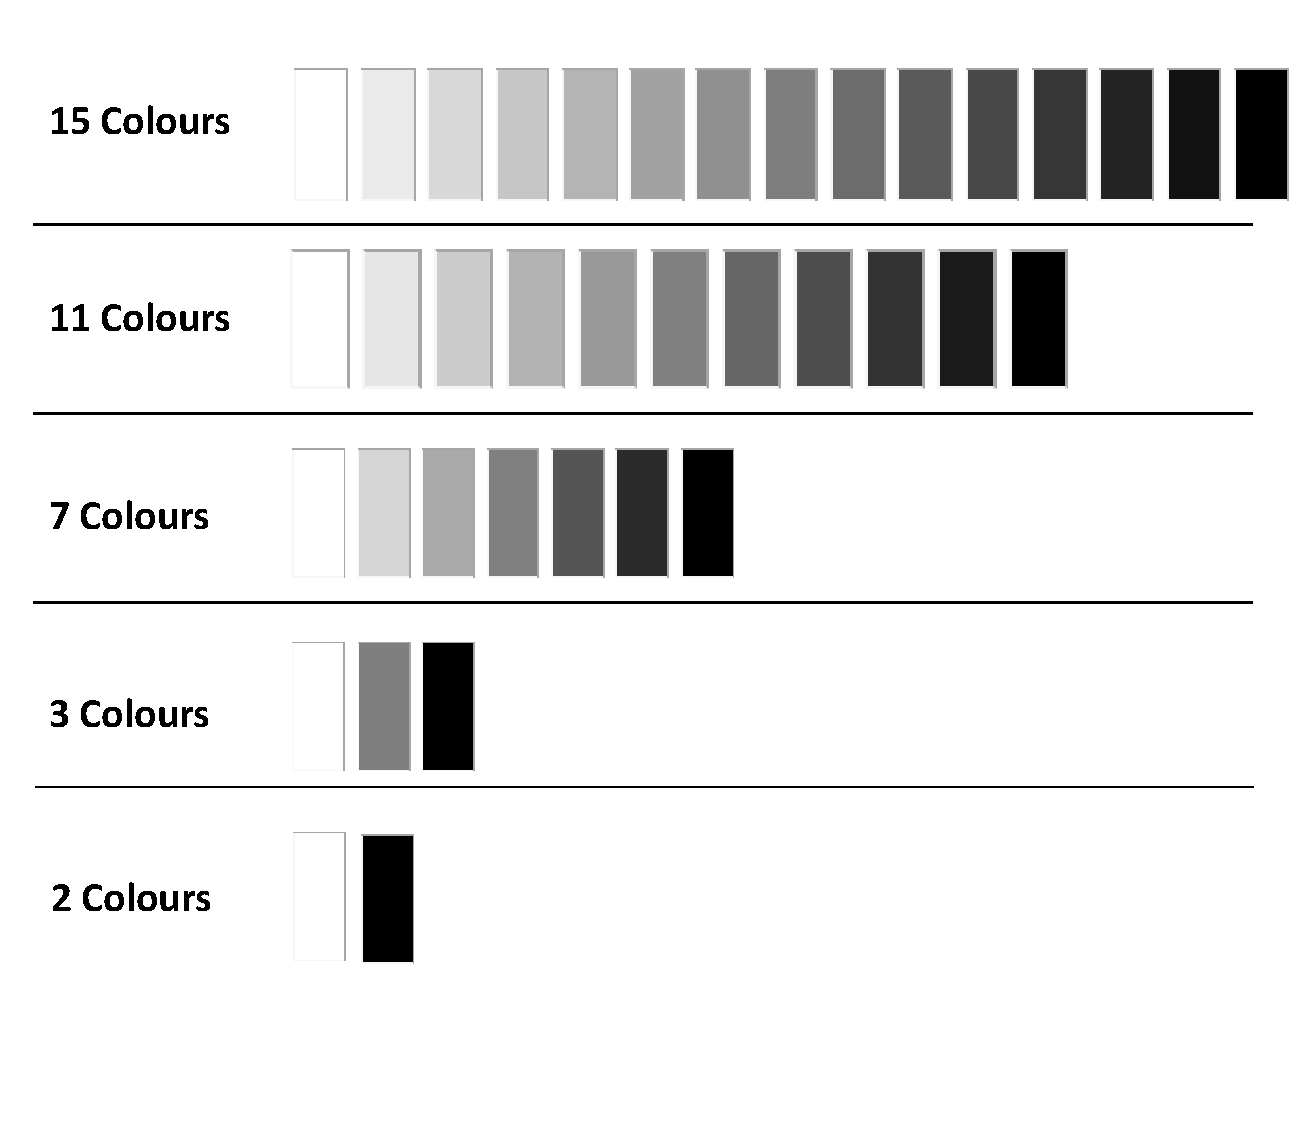
\includegraphics[width = 0.4\textwidth]{colourScheme.pdf}
\caption{Grey scale per number of colours}
\label{fig:colourScheme}
\end{center}
\end{figure} 

The colour scale is presented individually per treatment to the participant on the left of the interface (Figure \ref{fig:Interface}).
Participants can choose from 100 boxes for each round they play. The large number of boxes ensures an information overload, but still enables participants to achieve a satisfying result. The knapsack is illustrated as a wide rectangle and is limited by its width. Boxes can be added to and removed from the knapsack by clicking on them. In the cases that a selected box doesn't fit into the knapsack because it exceeds its capacity, the knapsack will shake and appear in red, not allowing the selected box to enter the knapsack. 
 \begin{figure}[htp] % Interface
\begin{center} %Exemplary interface
  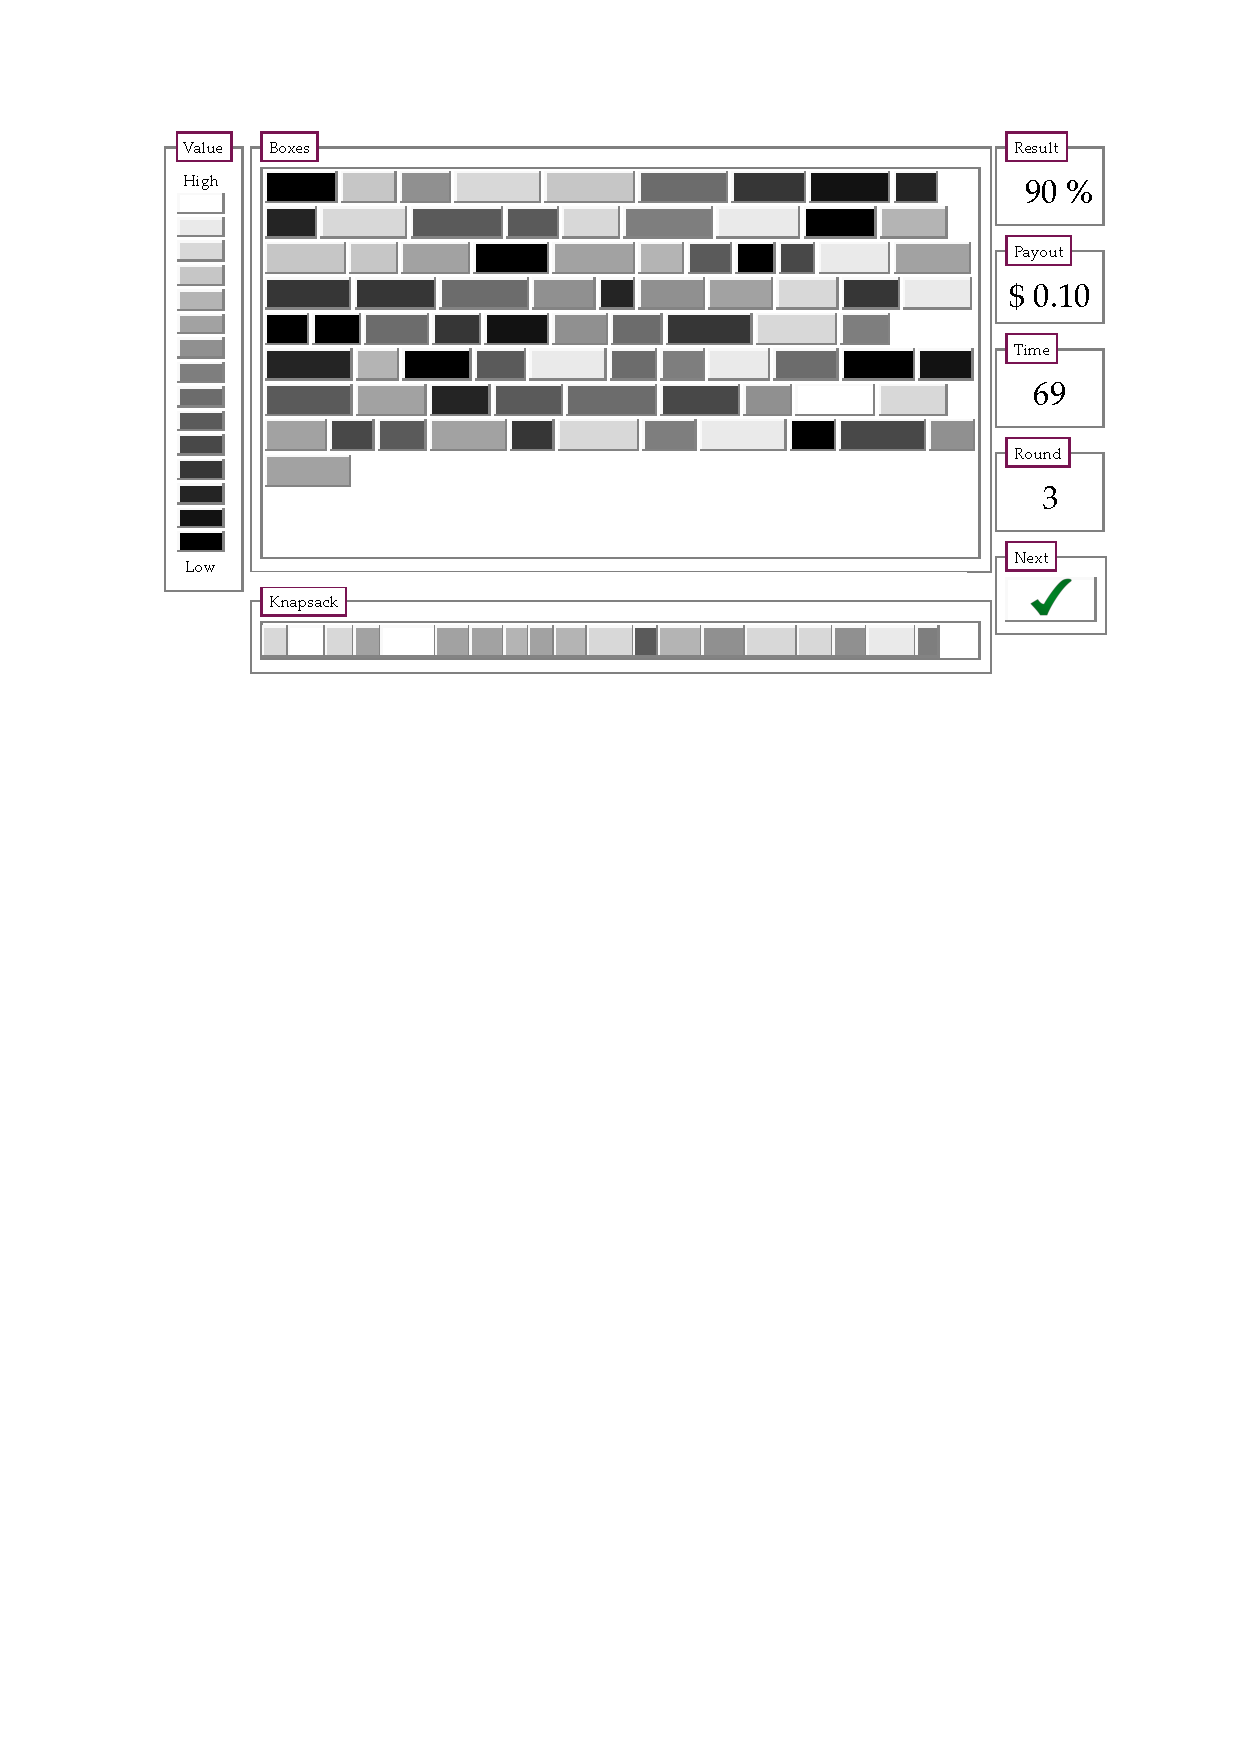
\includegraphics[height = 0.5\textwidth]{Interface4.pdf}
\caption{Exemplary interface (Treatment 5, Trial 1 )}
\end{center}
\label{fig:Interface}
\end{figure} 
\subsection{Description of the toolboxes}

\paragraph{Result}

The performance of the participants is measured by comparing the current value of the knapsack to the optimal solution calculated by the \ac{DPA} introduced in Section \ref{ch:Experiment:sec:Knapsack}.
  
\begin{equation}
x = \dfrac{\text{Current value of all boxes in knapsack}}{\text{\ac{DPA} solution }}
\label{eq:x}
\end{equation}

\paragraph{Payout}

In correspondence to the result, participants receive monetary compensation for playing the current round. Every time the bonus bar\footnote{Refer to Subsection \ref{ch:Experiment:sec:Interface:subsec:Payout scheme}.} is reached, the toolbox turns green to get the participant's attention to further work on improving the result.

\paragraph{Time}
The time restriction is set to 100 seconds per round. This rather long duration is chosen because participants should not experience a significant time pressure. The main goal is to isolate the colour effect; a potential time pressure effect is not the focus of the research since time has an impact on the decision quality \citep{Hahn2006}. A time limitation, however, must be implemented to ensure that it is necessary to play the round in one sitting (refer to subsection  \ref{ch:Experiment:sec:OnlineImplementation:subsec:AMT}).
The \textit{Next} button is available to give participants the opportunity to skip the current round when they have already reached a personally satisfying result and do not want to wait for the round to be finished.
\paragraph{Round}
Participants must complete three rounds. Multiple rounds are chosen to identify a potential learning effect; the limitation to three rounds keeps the total time for the experiment to a level that is attractive for an \acf{AMT} experiment. 


\subsection{Payout scheme}
\label{ch:Experiment:sec:Interface:subsec:Payout scheme}
The implemented payout scheme has two components – a guaranteed payout for each completed round and a payout dependent on the participant’s performance. A guaranteed payout is necessary to advertise the experiment on \ac{AMT} and an attractive offer draws a larger participant pool. The bonus leverage is increased in Trial 2 so the differences in the payout schemes must be taken into account in the analysis.

To ensure that participants do not only hit the \textit{Next}-button in each round and still get the minimum payout, a restriction is designed to only pay out participants who clicked at least one box per round.
 \begin{figure}[htp] % PayoutScheme
\begin{center}
\begin{subfigure} 
\centering
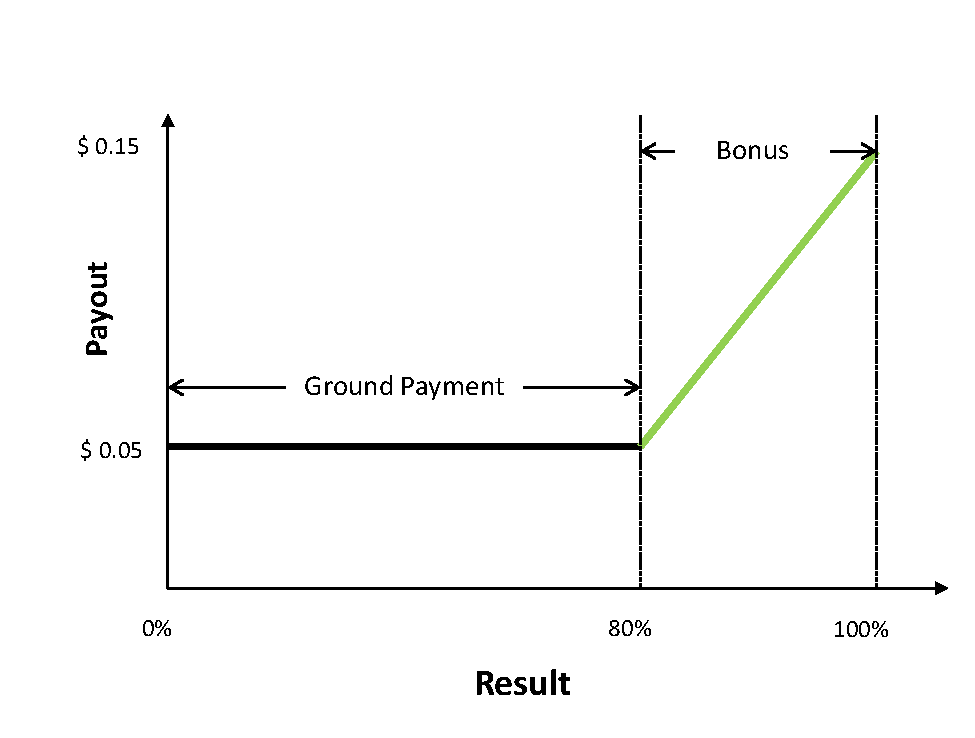
\includegraphics[height = 0.30\textwidth]{PayoutScheme.pdf}
\end{subfigure}
\begin{subfigure} 
\centering
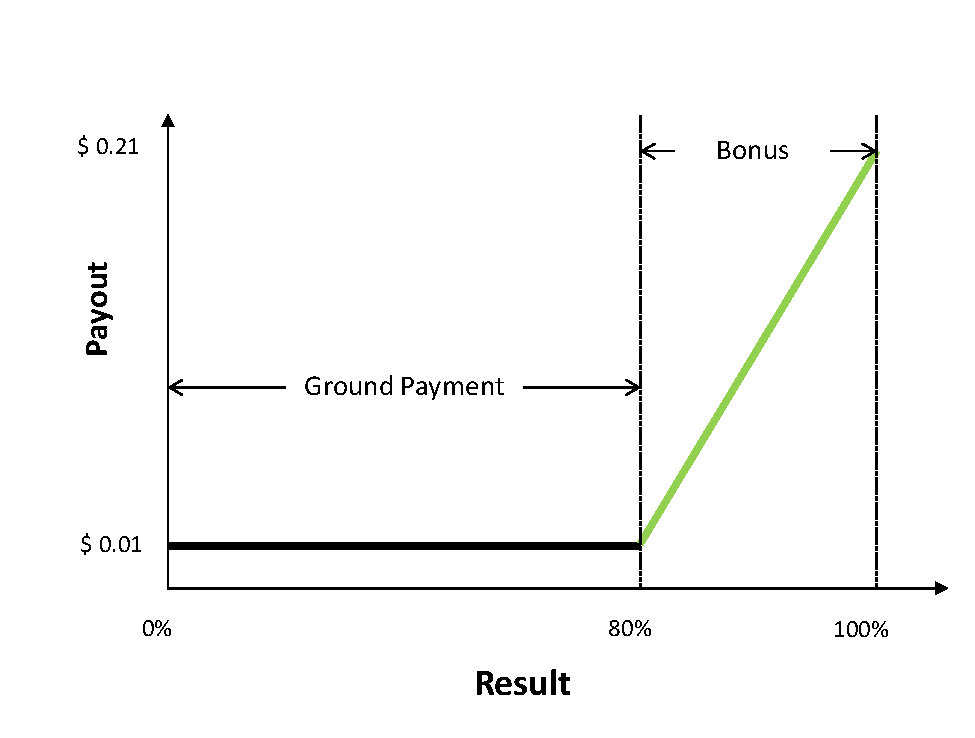
\includegraphics[height = 0.30\textwidth]{PayoutScheme2.pdf}
\end{subfigure}
\caption{Payout scheme for Trial 1 and 2}
\label{fig:PayoutScheme}
\end{center}
\end{figure} 

The reason for choosing a bonus system is to get participants to compare boxes of different weights and benefits and to make  them try different combinations for the knapsack.
In order to incentivize such behaviour, a bonus system can help. Trial rounds show that getting up to 80\% is possible when participants make an effort and try out different solutions. Hence, the performance incentive starts at 80\% and offers the participants in the first Trial an additional bonus of up to \$0.10 when reaching 100\%, resulting in a potential total payout of \$0.15 per round. Nevertheless, the experience of Trial 1 shows a large number of participants who did not reach the bonus bar. Therefore, we increased the leverage of the bonus system in Trial 2, from a ground payment of \$0.01 to a possible total payout of \$0.21 when reaching 100\%.

%% ===========================
\section{Online Implementation}
\label{ch:Experiment:sec:OnlineImplementation}
%% ===========================

For the setup of an online environment, the Python web framework Django 1.4.3 is used to implement the communication between \ac{GUI} and the server.
The experiment is advertised on \acf{AMT} as a \ac{HIT}.

\subsection{\acl{AMT}}
\label{ch:Experiment:sec:OnlineImplementation:subsec:AMT}
A previous research study \citep{Schmidt2012} using a similar interface and setup reached 28 participants. While the results helped to prove that more colours to choose from does not increase the average payout, the overall experiment lacked a wider statistical foundation.
Consequently, we try to increase the foundation by using the online labour market \acf{AMT}.

The \ac{AMT} platform is the most active online labour market for conducting behavioural experiments. It enables researchers to conduct experiments very quickly, cheaply \citep{Rand2012}, and in good quality \citep{Gardner2012}. Moreover, the data gained is at least as reliable as the data obtained via traditional methods \citep{Buhrmester2011}. \ac{AMT} connects employers with potential workers who are paid according to the satisfactory completion of the assigned task. Furthermore, workers can be motivated to perform well by a bonus structure. Since individuals can participate entirely over the computer, the experience is quite similar to participating in computer simulations.

Researchers can act as employers on the \ac{AMT} website by offering experiments as tasks otherwise known as a \acf{HIT}. Completing an \ac{HIT} usually results in a payment of less than \$1.00 for less than 5 minutes of work. Users are from around the world, but are mainly concentrated in the United States and India \citep{Rand2012}. These findings are supported by our experiences.

\paragraph{Limitations of \acl{AMT}}
Although the \ac{AMT} offers a promising potential for the purposes of our study, there are several limitations to keep in mind.

First, in contrast to experiments conducted in a lab environment, \ac{AMT} experiments have limited control over what kind of individuals take part in the experiment. In particular, the lack of control over \textit{non-random attrition} \citep{Rand2012} defines a limitation for our experiment in terms of the participant structure. Individuals who are overwhelmed with the complexity of the task might drop out early, not finish the \ac{HIT} and may not be included in the statistical analysis. This can have an impact on the pool of participants among different treatments and can therefore limit our ability to compare results. As a result, we have tried to make the description of the game and the game itself as simple and intuitive as possible in order to reduce the risk of early drop-outs. Test runs previous to offering the \ac{HIT} revealed that using the Test round helped individuals to get a better understanding of the game and the task.

Second, researchers cannot be sure what participants are actually doing during the experiment on the \ac{AMT} platform. This fact especially reduces the benefit to cognitive load experiments similar to our experiment since our experiment necessitates the full attention of each individual. We try to tackle this issue by setting a time restriction per round so individuals have an incentive to stay on task. Moreover, we log the time that individuals spend on different parts of the experiment and evaluate the participant's actions by analysing the recorded data. We are therefore able to better understand each individual's actions. Lastly, we take this limitation into consideration in the choice of a statistical model.

Third, the statistical analysis is based on the assumptions that every observation is independent. In the setup of our experiment, individuals are able to conduct the experiment over and over by re-directing to the start page after finishing a session. Even though repeat responses appear to be a minor concern according to \cite{Berinsky2012}, it can still potentially dilute the observation independence and the statistical value of the learning effect. We therefore record the IP address of each user when they are directed to the welcome page in order to exclude those participants who play several games successively. However, this method does not exclude those individuals who change their IP in-between experiments.
Moreover, the \ac{AMT} platform has other disadvantages against a lab experiment in terms of user support during the experiment, and the lack of control over the English language competencies of individuals. 

After summarizing the benefits and limitations of the \ac{AMT} platform, we conclude that \ac{AMT} is feasible for our experiment when the design and evaluation of the experiment takes the limitations into consideration.

\subsection{System design}

\cite{Rand2012} indicates that in order to conduct an experiment using a game environment on \ac{AMT}, researchers must provide participants with instructions, making sure they understand the rules of the game. Next, researchers must process the data and pay the participants according to their earnings. We follow this setup for our experiment (refer to Figure \ref{fig:Enfolab}).

Once the \ac{AMT} user has decided to complete the \ac{HIT}, he or she is redirected to an external web page on which the experiment is run.
When arriving at the page, the program creates an individual user who is randomly assigned to one treatment and an individual code is generated. 
Additionally, a time stamp is saved in order to track the time a user will spend on different stages throughout the experiment.

\afterpage{
\begin{landscape}
\begin{figure}[htbp] % DistributionBestResult
\begin{center} 
\caption{Design of the online environment}
\label{fig:Enfolab} 
\begin{subfigure} 
\centering
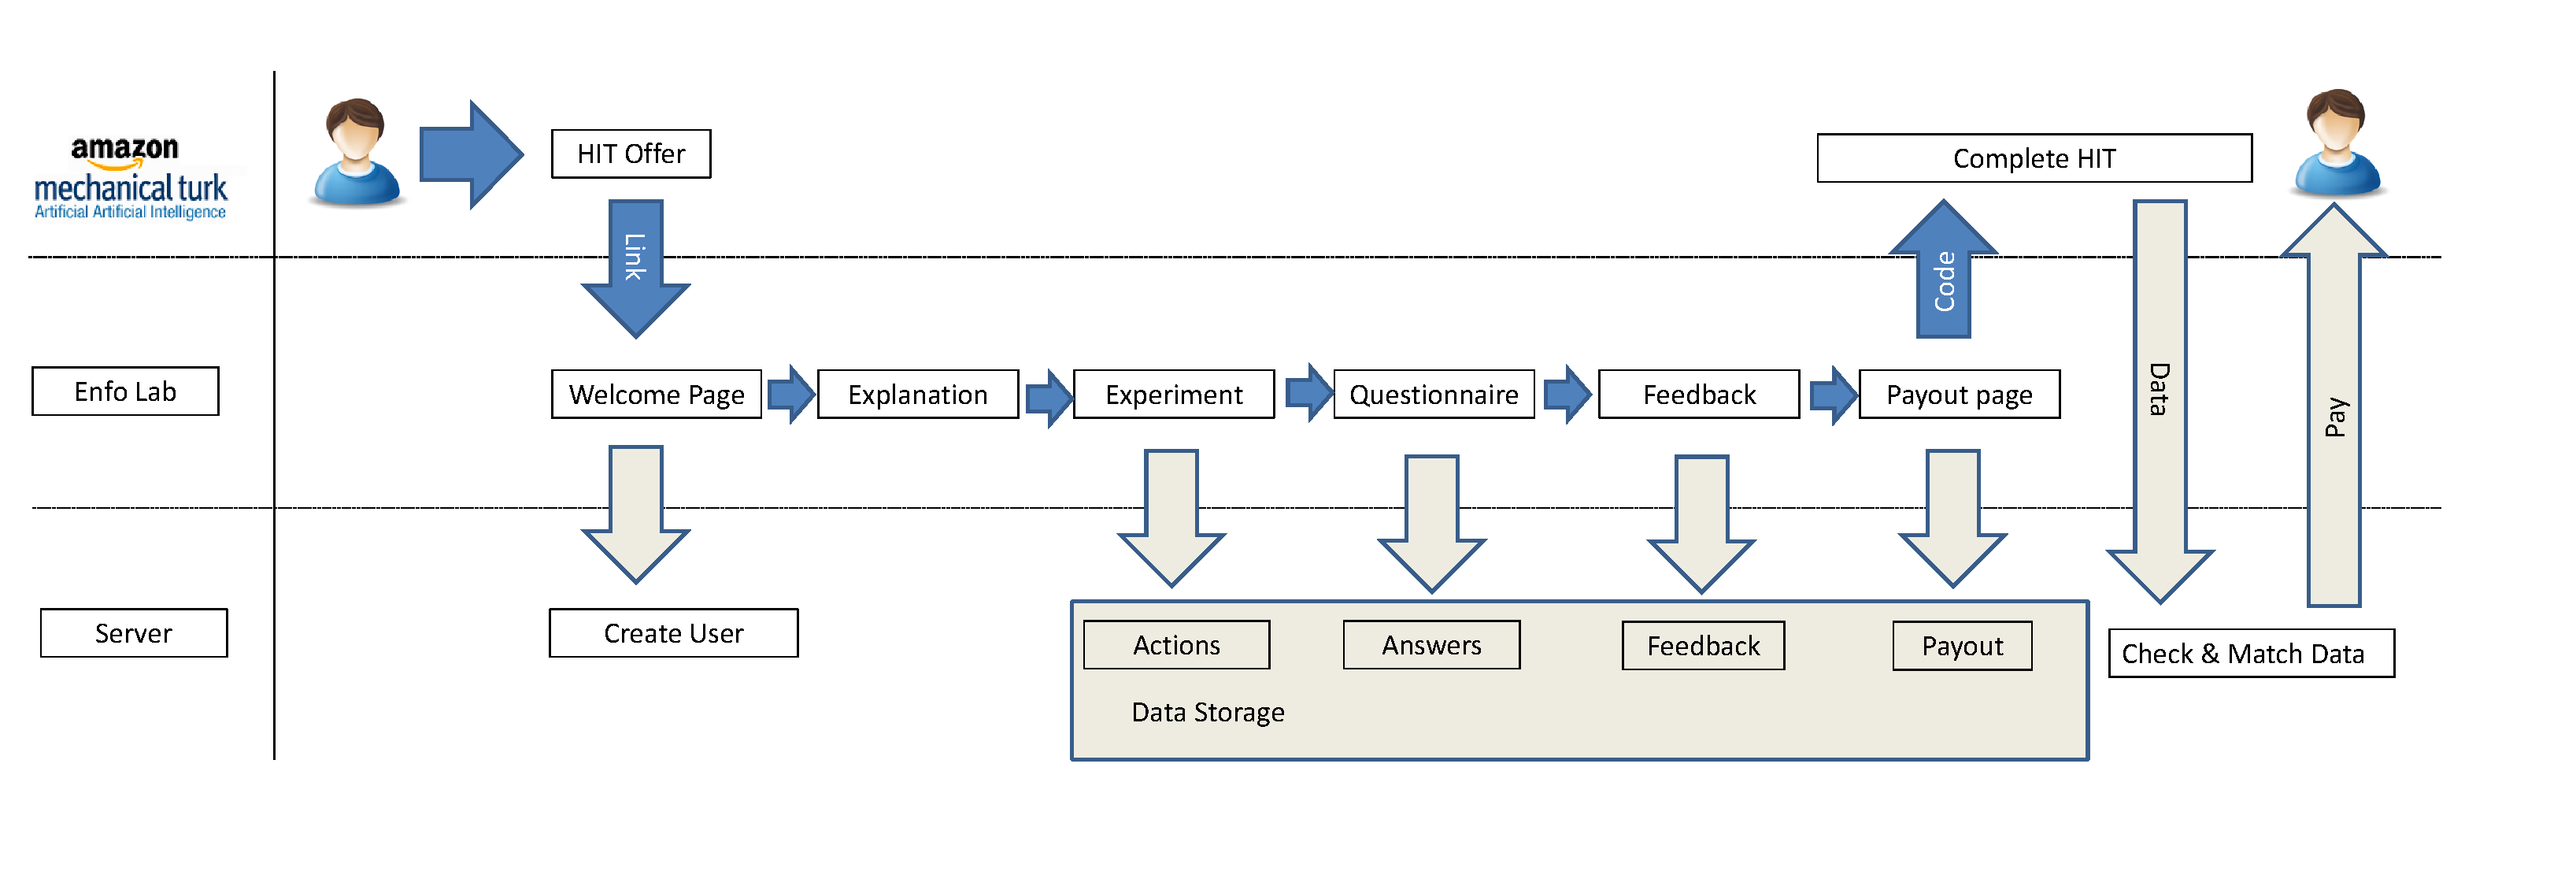
\includegraphics[width = 1.5\textwidth]{EnfoLab_Coordination.pdf}
\end{subfigure} 
\begin{subfigure} 
\centering
  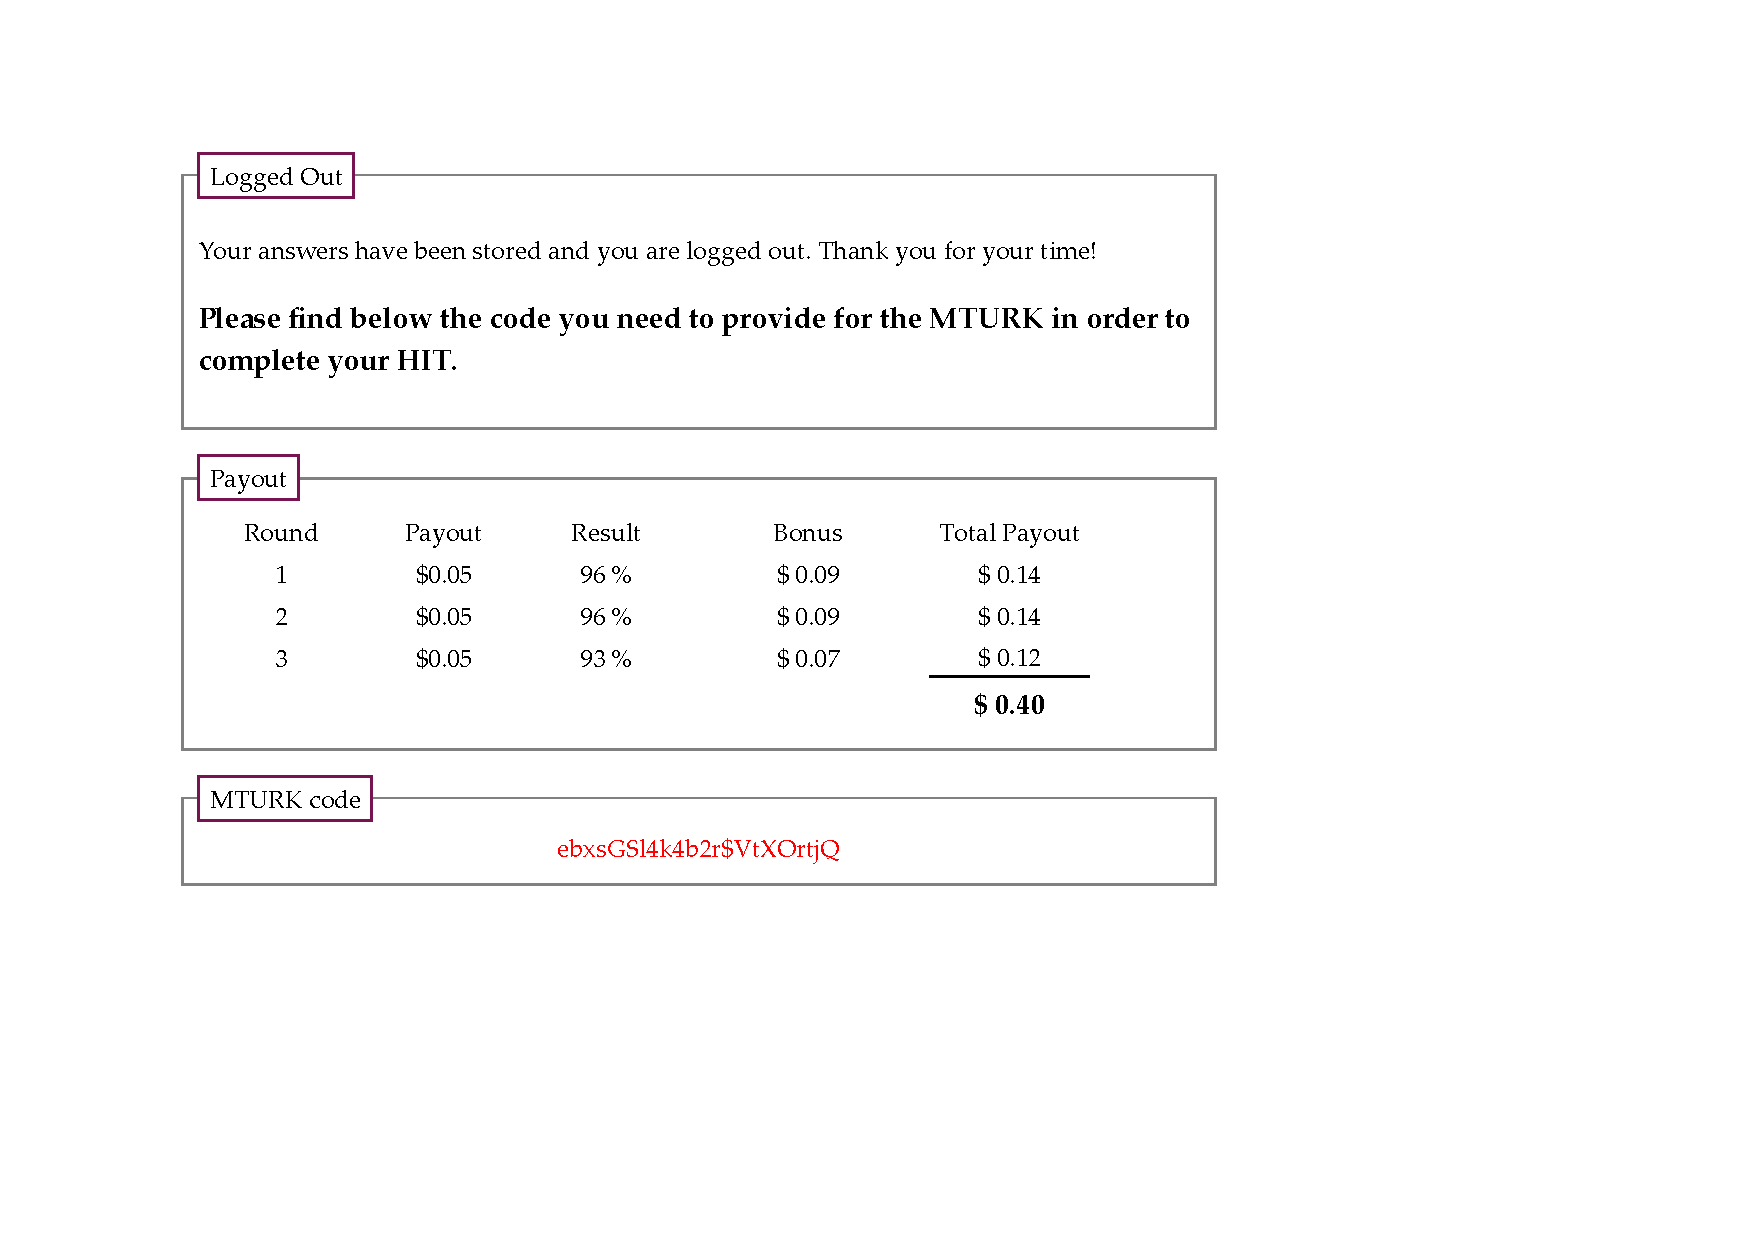
\includegraphics[height = 0.5\textwidth]{PayoutView.pdf}
\end{subfigure}
  \caption{Final page with payout}
    \label{fig:FinalPage} 
\end{center}
\end{figure}
\end{landscape}}
The participants first go through the explanation of the game where they are introduced to the concept of the knapsack problem and the implemented graphical interface. 
Before the participants begin playing their three rounds, they can get used to the interface by playing a Trial round which has no time restriction and offers information boxes to explain the different parts of the interface.

The participants then start the game by playing the three rounds of the experiment. Every action that includes adding or removing a box to or from the knapsack is saved on the server, including time, box ID, box benefit, box weight, current payout, the type of action (remove or add) and whether or not the knapsack is full.
The \ac{JSON} is used to transfer the determined data to the server. The collected data can be extracted from the server via a \ac{CSV} file.

After completing the game, participants are presented with a questionnaire where they must answer six questions about their experience playing the game and the strategy they used. To avoid participants rushing through the questionnaire, a minimum time of 15 seconds is introduced. If participants spend less time on the questionnaire, they are redirected to the beginning of the questionnaire. In addition, we include an additional question in Trial 2 that is directed to evaluate the participant's attention, by asking them to give a specific answer to the question.

Subsequent to the questionnaire, participants have the opportunity to give feedback by filling in a text box. This feedback is used to have an additional feedback channel to identify problems in any aspect of the interface. The final payout for the experiment (Figure \ref{fig:FinalPage}) is shown to the participants after they have completed their three rounds and the questionnaire.

When the minimum requirement of clicking at least one box per round is fulfilled, participants are presented the payout for each round and the total payout. Furthermore, the \ac{AMT} code is provided. The user then goes back onto the \ac{AMT} system, enters the \ac{AMT} code and completes his or her \ac{HIT}. At the end, the data on the server is compared to the \ac{HIT}s completed, and the payout is made via the \ac{AMT} system.

%% ===========================
\section{Data Acquisition}
\label{ch:Experiment:sec:DataacquisitionDescriptives}
%% ===========================
The 1\textsuperscript{st} Trial was offered on \ac{AMT} between the 20\textsuperscript{th} and the 21\textsuperscript{st} of February 2013 and reached 200 participants, the 2\textsuperscript{nd} Trial with the same amount of participants ran between the 5\textsuperscript{th} and the 8\textsuperscript{th} of March 2013. A total of 31.291 clicks on boxes were recorded on the server.


Before the data is statistically analysed using IBM's \textbf{SPSS} as well as the free alternative \textbf{R}, the recorded data is cumulated on a per round basis for the purposes of this study. For each round per user, a data point is created that includes information on the user, treatment and corresponding number of colours, round, number of decisions, first result, best result, final result and finally the time for each result.
 \begin{figure}[htp] % Interface 1
\begin{center} %Exemplary interface
  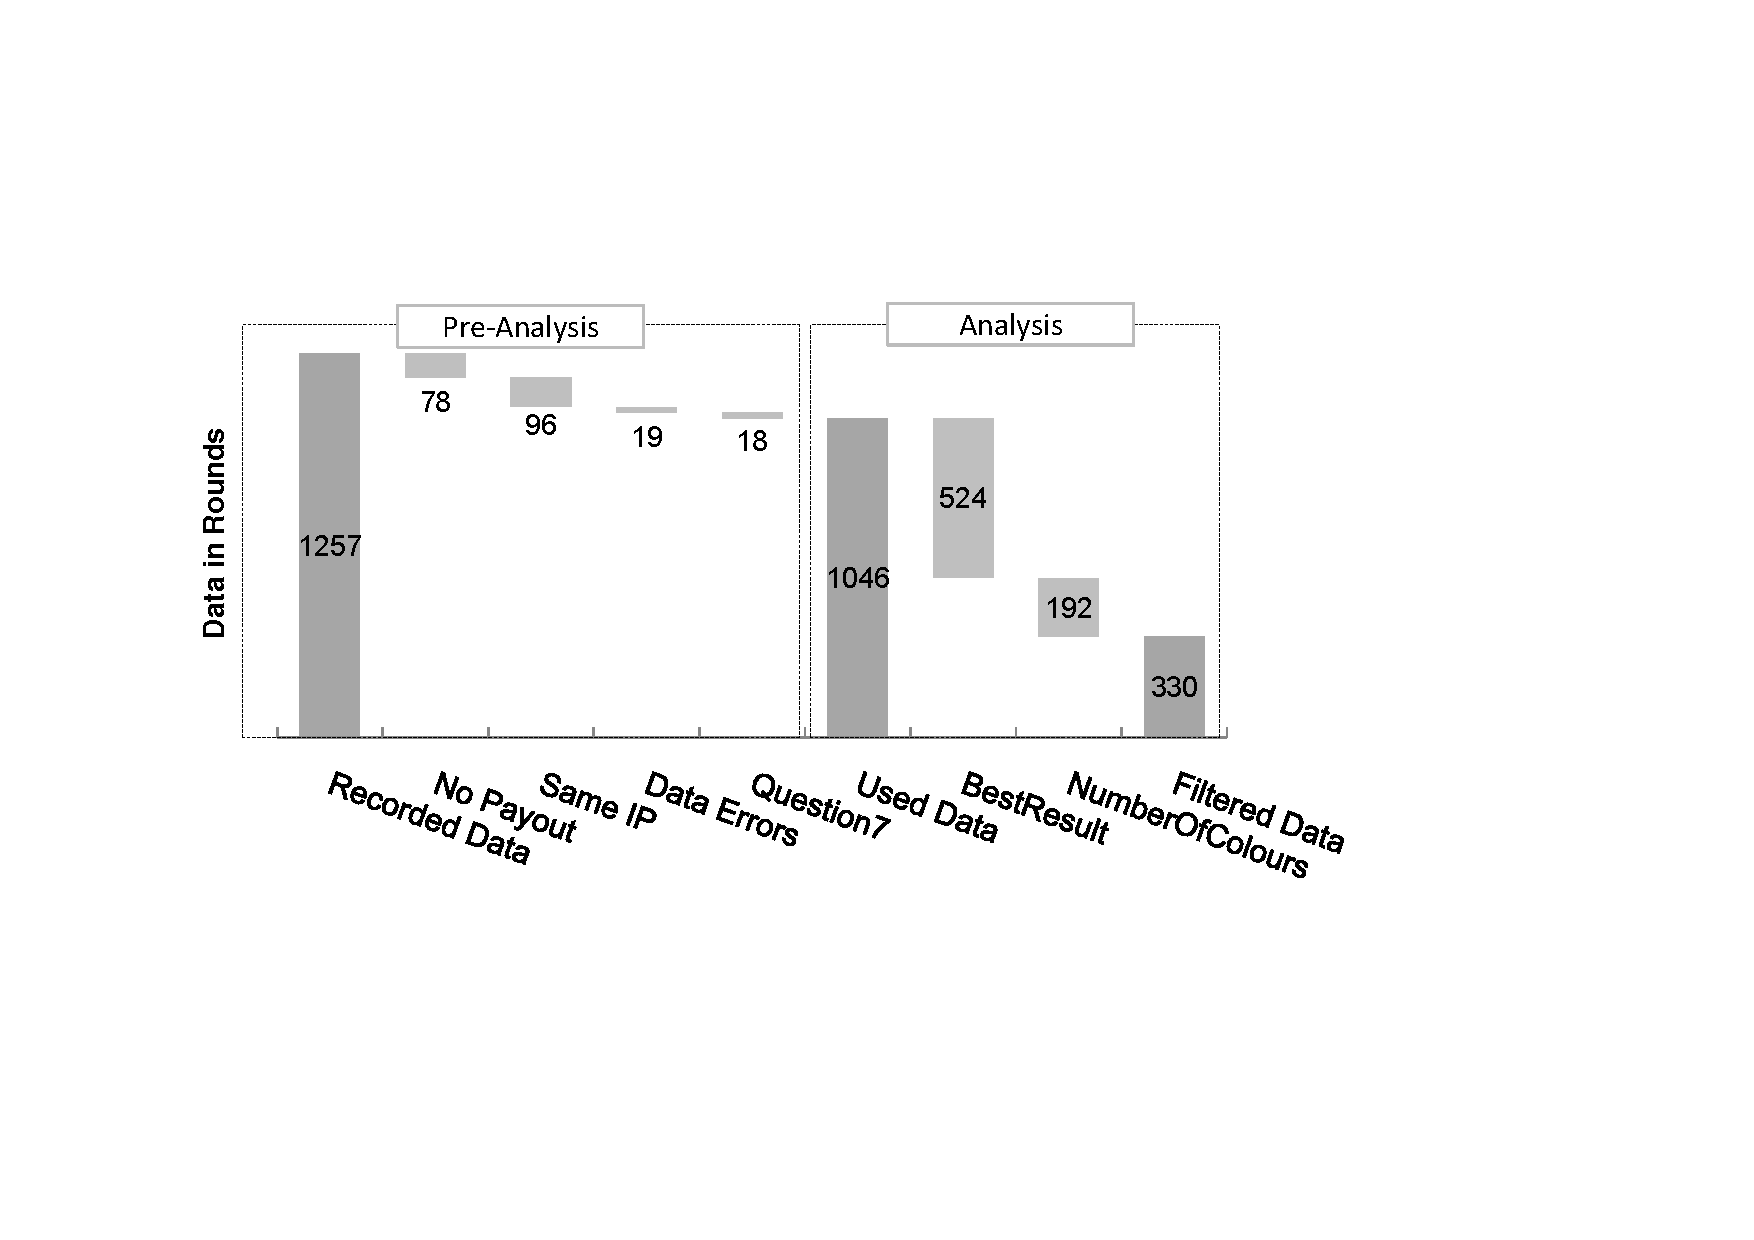
\includegraphics[height = 0.5\textwidth]{User_Waterfall.pdf}
  \caption{Generated Data in Rounds}
  \label{Data}
\end{center}
\end{figure}
Out of a potential 1.200 rounds per 400 participants, there are 1.257 played rounds recorded (refer to Figure \ref{Data}). The fact that the recorded number of rounds outnumbers the potential 1.200 rounds, can be explained using two cases: first by the functionality test rounds conducted by the research team while the game was running and second by participants playing one or two rounds, then dropping out of the experiment. These cases can be identified by looking at the payout of the user, since there was no payout made to users who did not complete all rounds. Consequently, we will exclude the rounds of those users who did not achieve a payout greater than 0.

The next step is to identify the users who played the game again and again, and therefore have skewed the observation independence as described in Section \ref{ch:Experiment:sec:OnlineImplementation:subsec:AMT}. 32 users are found who share both their IP with at least one other user and who achieved a payout greater than 0. We do not exclude those users who committed only once to the experiment and therefore only reached a payout greater than 0 once.

The data of 6 participants showed errors, e.g. a total game time per round greater than 100s or a result greater than 100\%. Since we were not able to trace the origin of these errors, we will exclude these users from the data set.
As a result, 349 users with a total of 1.046 rounds build the data for the statistical analysis.

Within the data used for the analysis, there are two further filters applied.
These filters are used to focus on the participants who made an effort to succeed in the game. As stated in Section \ref{ch:Experiment:sec:DataacquisitionDescriptives:subsec:DescriptiveStatistics}, a performance lower than 80\% per round can be explained by a lack of effort or understanding on the participant's side. By including the whole range of performances in the parameter estimation, the statistical noise might dilute the inductive value of the study. Consequently, we only concentrate on participants who were able to achieve a result greater than or equal to 80\% for each round. This filter leaves a data set consisting of 174 users with a total of 522 rounds recorded. We will refer to this filter as \textbf{Filter 1}.

In a second step, users who are assigned to a treatment group with less than 7 colours are excluded. This is due to statistical implications of the data since significant results can be seen for the three remaining treatments. After applying both filters, the data set is made up of 110 users with 330 rounds recorded. We will refer to this data set as \textbf{Filter 2}.

The different filters will be subsequently applied for the statistical analysis.
%
%
%Before starting the analysis, an additional implication of \acf{AMT} is taken into consideration. Cognitive load experiments conducted to the \acf{AMT} platform run the risk that users might not commit their full attention on the task (rf. to Section \ref{ch:Experiment:sec:OnlineImplementation:subsec:AMT}) and therefore may experience a different information overload than the users who give their full attention to the task. We try to determine these users by looking at the time it takes them to fill up the knapsack for the first time. Users who just randomly select boxes and quickly fill up the knapsack have a very low time until they first reach a full knapsack. A time border of 5 seconds is chosen to separate these users and the filtered data is excluded from the data set.
%Our final data set includes 536 recorded rounds from 180 users, and includes 12.929 actions.
%
%
%
%

%% ===============================
\paragraph{Experiment stages}
%% ===============================
 \begin{figure}[htbp] % Timelog
\begin{center} %Timelog
  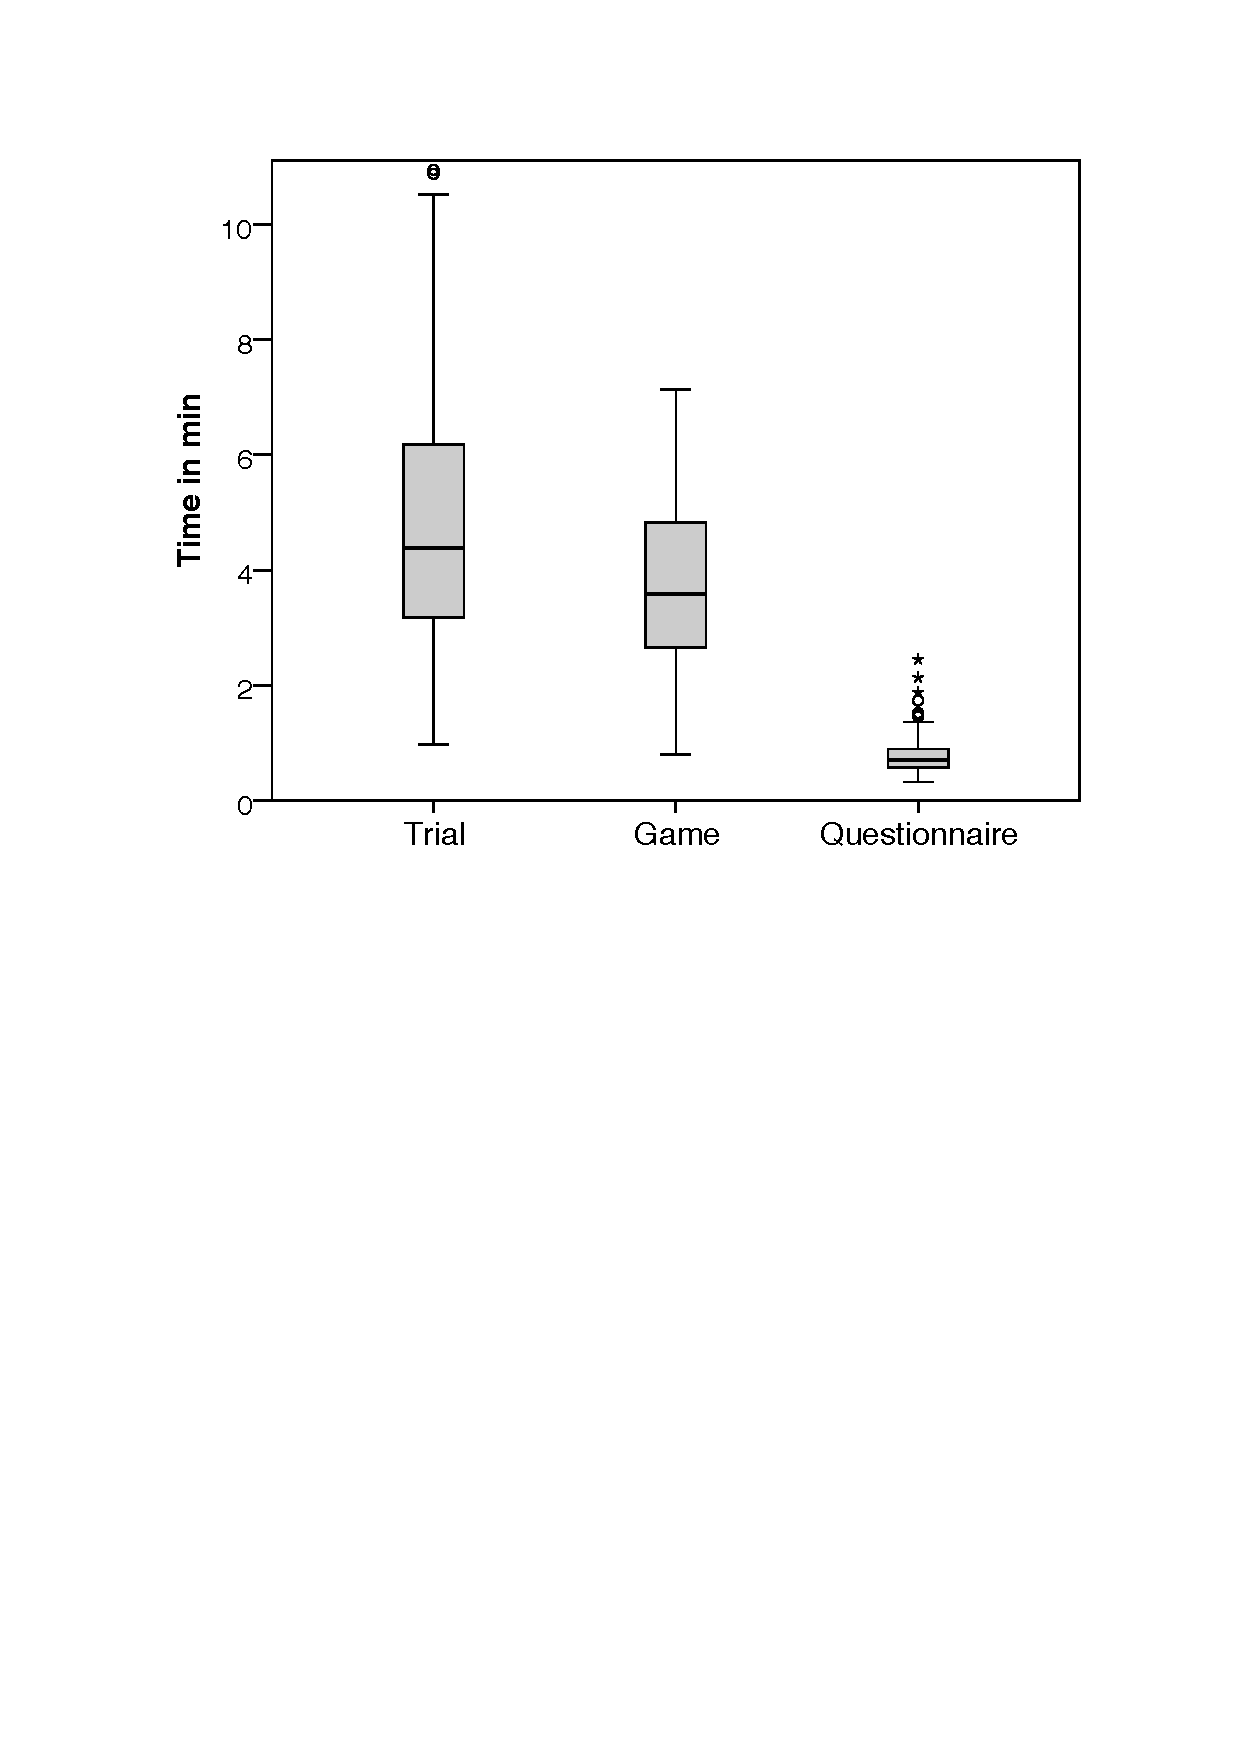
\includegraphics[height = 0.4\textwidth]{Timelog.pdf}
  \caption[Time spent on different stages of experiment]{Time spent on different stages of experiment\footnotemark}
  \label{Time spent on different stages of experiment}
\end{center}
\end{figure}
\footnotetext{Outliers with a time greater than 11 minutes on each stage are excluded for the purposes of this graph due to better readability. }

The tracked time logs for the participants  (Figure \ref{Time spent on different stages of experiment}) show that individuals spent a considerable amount of time on the explanation and the Trial round. The total game length is defined by 5 minutes, and the majority of participants complete the game in less than the maximum time. A value greater than 5 minutes can be explained by the information box that pops up before the beginning of the game. The countdown for the current round only starts after participants click on the information box to start the round, resulting in a total game duration longer than 5 minutes when participants do not click instantly on the info box.
The questionnaire is the shortest of the stages. We set a minimum time of 15 seconds, corresponding to 0.25 minutes, to fill out the questionnaire - the majority of individuals spent between 30 and 60 seconds on the questionnaire section.

%% ===============================
\paragraph{Feedback from participants}
53\% of all users used the opportunity to give feedback via text. The majority gave positive feedback on the technical functionality of the game. These results might, however, be skewed since the feedback page is only reached by participants who did not have any major technical problems while going through the experiment.

Only a small number of participants gave feedback on areas of improvement, including the suggestion to offer a better and earlier visual notification when the time is running out. One participant suggested to introduce a more colourful colour scale or background music.


%% ===============================
\section{Data Descriptives}
\label{ch:Experiment:sec:DataacquisitionDescriptives:subsec:DescriptiveStatistics}
%% ===============================

This section aims to provide a descriptive overview of the unfiltered data. First, the treatment statistics are introduced, second the descriptive results from the game are analysed and third the answers from the participants are examined.
%% ===============================
\paragraph{Treatments and payout}
\label{ch:Evaluation:sec:DescriptiveStatistics:subsec:Distributionoftreatments}

The participants were randomly and uniformly assigned to one treatment once they directed to the welcome page. The low share of treatment 1 is related to the fact that the treatment was added in Trial 2 (Table \ref{Distributionoftreatments}).

\begin{table}[htbp] % Distribution of treatments
  \centering
  \caption{Distribution of Treatments}
    \label{Distributionoftreatments}
    \begin{tabular}{ccccc}
    \toprule
    \multirow{2}[1]{*}{Treatment} & \multirow{2}[1]{*}{Users} & \multirow{2}[1]{*}{Share} & Share of  & Share\\
    						   &						&  						 &	Dropouts\footnotemark & Minimum Payout\\
    \midrule
    1     & 33    & 10\%  & 37\% & 31\%\\
    2     & 88    & 25\%  & 40\% & 25\%\\
    3     & 78    & 22\%  & 40\% & 31\%\\
    4     & 72    & 21\%  & 39\% & 28\%\\
    5     & 77    & 22\%  & 46\% & 27\%\\
    
    \bottomrule
    Total & 348   & 100\% & 40\% & 28\%\\
    \end{tabular}%
\end{table}%
\footnotetext{See Appendix \ref{Appendix-Formulas} for the formulas.}

The distribution of the payout presented in Figure \ref{Distributionofpayout} shows that the medians of the payout per treatment are decreasing with the \textit{NumberOfColours} in Trial 1, whereas an inverted U-Shape can be detected for the medians in Trial 2, with a peak at the medium 7-colour level.

28\% of all users achieved the minimum payout for each Trial, and 72\% reached the bonus bar. The highest payout is \$0.44 accomplished in Trial 1, and \$0.55 in Trial 2. 
 \begin{figure}[t] % Distributionofpayout
\begin{center} 
  \caption{Distribution of payout among treatments for each Trial}
  \label{Distributionofpayout}
  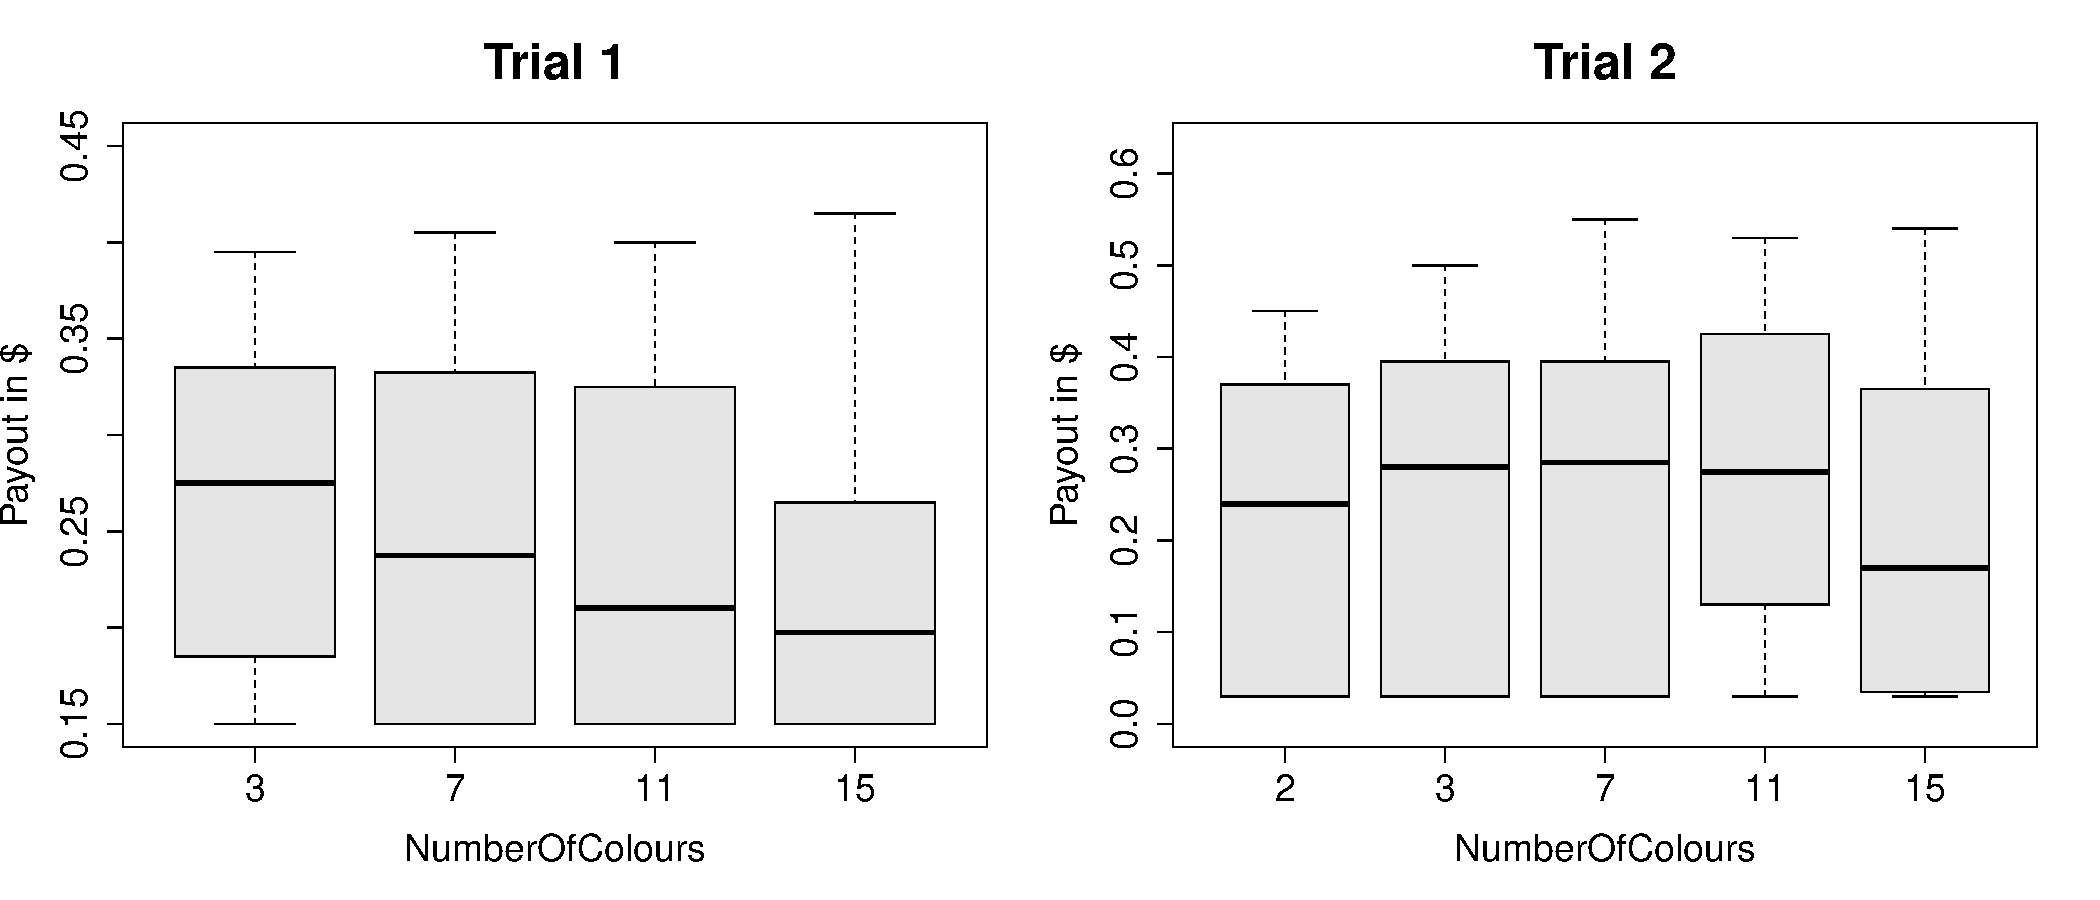
\includegraphics[width = 1\textwidth]{DescriptivesPayout.pdf} 
\end{center}
\end{figure}

The fact that the distribution of the payout seems to be differently distributed among trials can be explained by the different payout scheme, and does not indicate a different distribution of the underlying variable, the FinalResult, according to the trial assignation (Figure \ref{Distributionofpayout}) .
%% ===============================
\paragraph{Performance}
\label{ch:Evaluation:sec:DescriptiveStatistics:subsec:Performance}
As will be shown in Section 4, the trial assignation does not have an influence on the performances of the individual. Therefore, we now combine the results for both trials in the description of the data.
\begin{figure}[htbp] % DistributionFinalResult
\begin{center}
  \caption{FinalResult - Histogram and Box plot}
    \label{DistributionFinalResult} 
  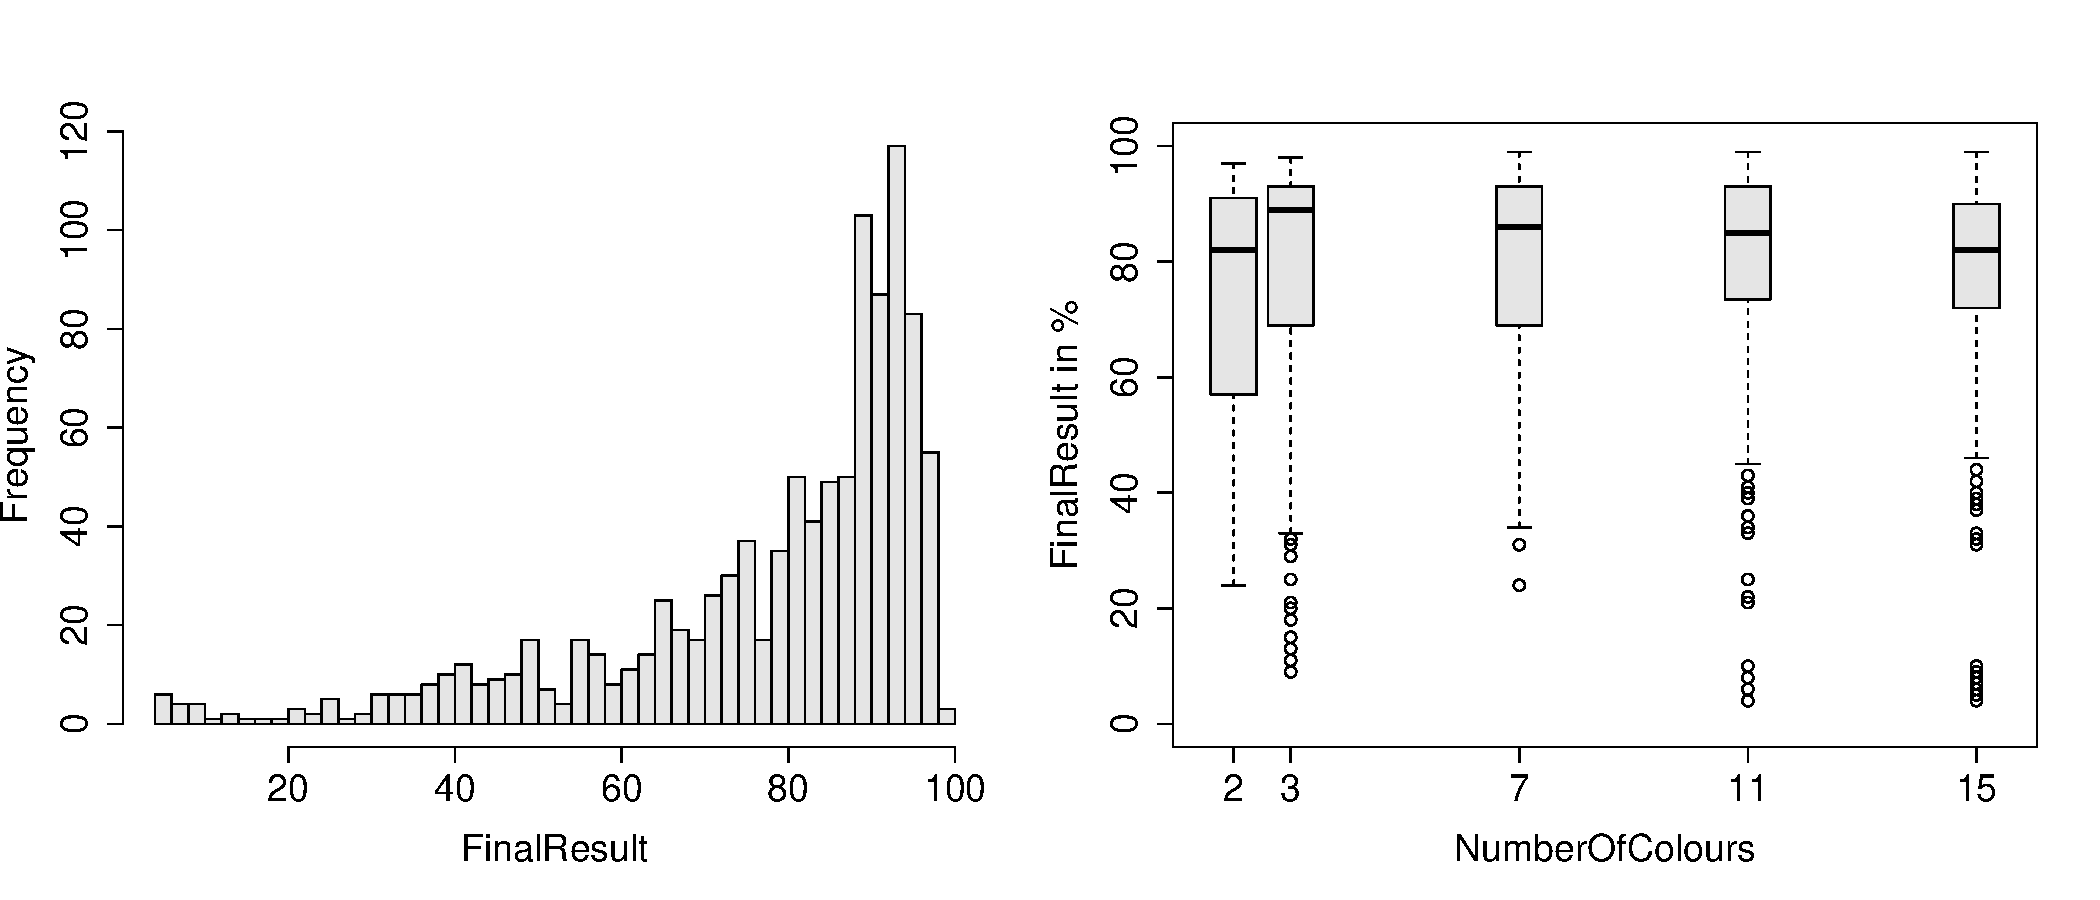
\includegraphics[width = 1\textwidth]{DescriptivesFinalResult.pdf}
\end{center}
\end{figure}
The characteristics of the histograms for all result types show a similar shape\footnote{Figure \ref{DistributionFinalResult} (left) shows the histogram for the \textit{FinalResult}, see Appendix \ref{Appendix-Descriptive} for Histograms and Boxplots for \textit{FirstResult} and \textit{BestResult}.}. The average result lies between 75\% for the \textit{FirstResult} and 79\% for the \textit{BestResult}. The relative standard deviation is high with values greater than 23\%, and the standard deviation is just below 20. 
The population for all result types is negatively skewed with a value between --1.29 and --1.58, and the kurtosis is positive in the range of 1.4 to 2.4. The modal group can be found between 85\% and 95\%.

As indicated by the histograms, there is a lot of noise in the data, since values below 80\% are likely to be related to a minimum effort. Therefore, the statistical potential is emphasized by excluding the low performers.
The distribution of the different result types among different treatments is exemplary shown in Figure \ref{DistributionFinalResult} (right) for the \textit{FinalResult} and indicates a decreasing interquartile range with an increasing number of colours. The medians for all treatments are above the bonus bar and show a tendency to form a U-Shape with a peak at the treatment with three colours.

Significant outliers can be found in all treatments except for the treatment with two colours. Outliers with a \textit{FinalResult} lower than 20\% can be explained by a lack of effort and understanding on behalf of the participant, as opposed to an experience of information overload. A result greater than this value can namely be achieved by simply clicking on random boxes to fill up the knapsack.
\paragraph{Time}
\label{ch:Evaluation:sec:DescriptiveStatistics:subsec:Time}
The histograms of the different time types differ. Whereas \textit{FirstTime} shows a positively skewed distribution, \textit{BestTime} seems to be closer to a uniform distribution. \textit{FinalTime} has a negatively skewed population and \textit{DecisionTime} looks like the results are normally distributed. The majority of participants reached the \textit{FirstResult} in under 40 seconds, and finished the round mostly in over 80 seconds. Since only a minority played the full time, the use of the "Next"-button seemed to be popular. No specific time can be identified when participants were most likely to reach their \textit{BestResult}.
\begin{figure}[htbp] % DistributionFinalTime
\begin{center}
  \caption{FinalTime - Histogram and Box plot}
   \label{DistributionFinalTime} 
 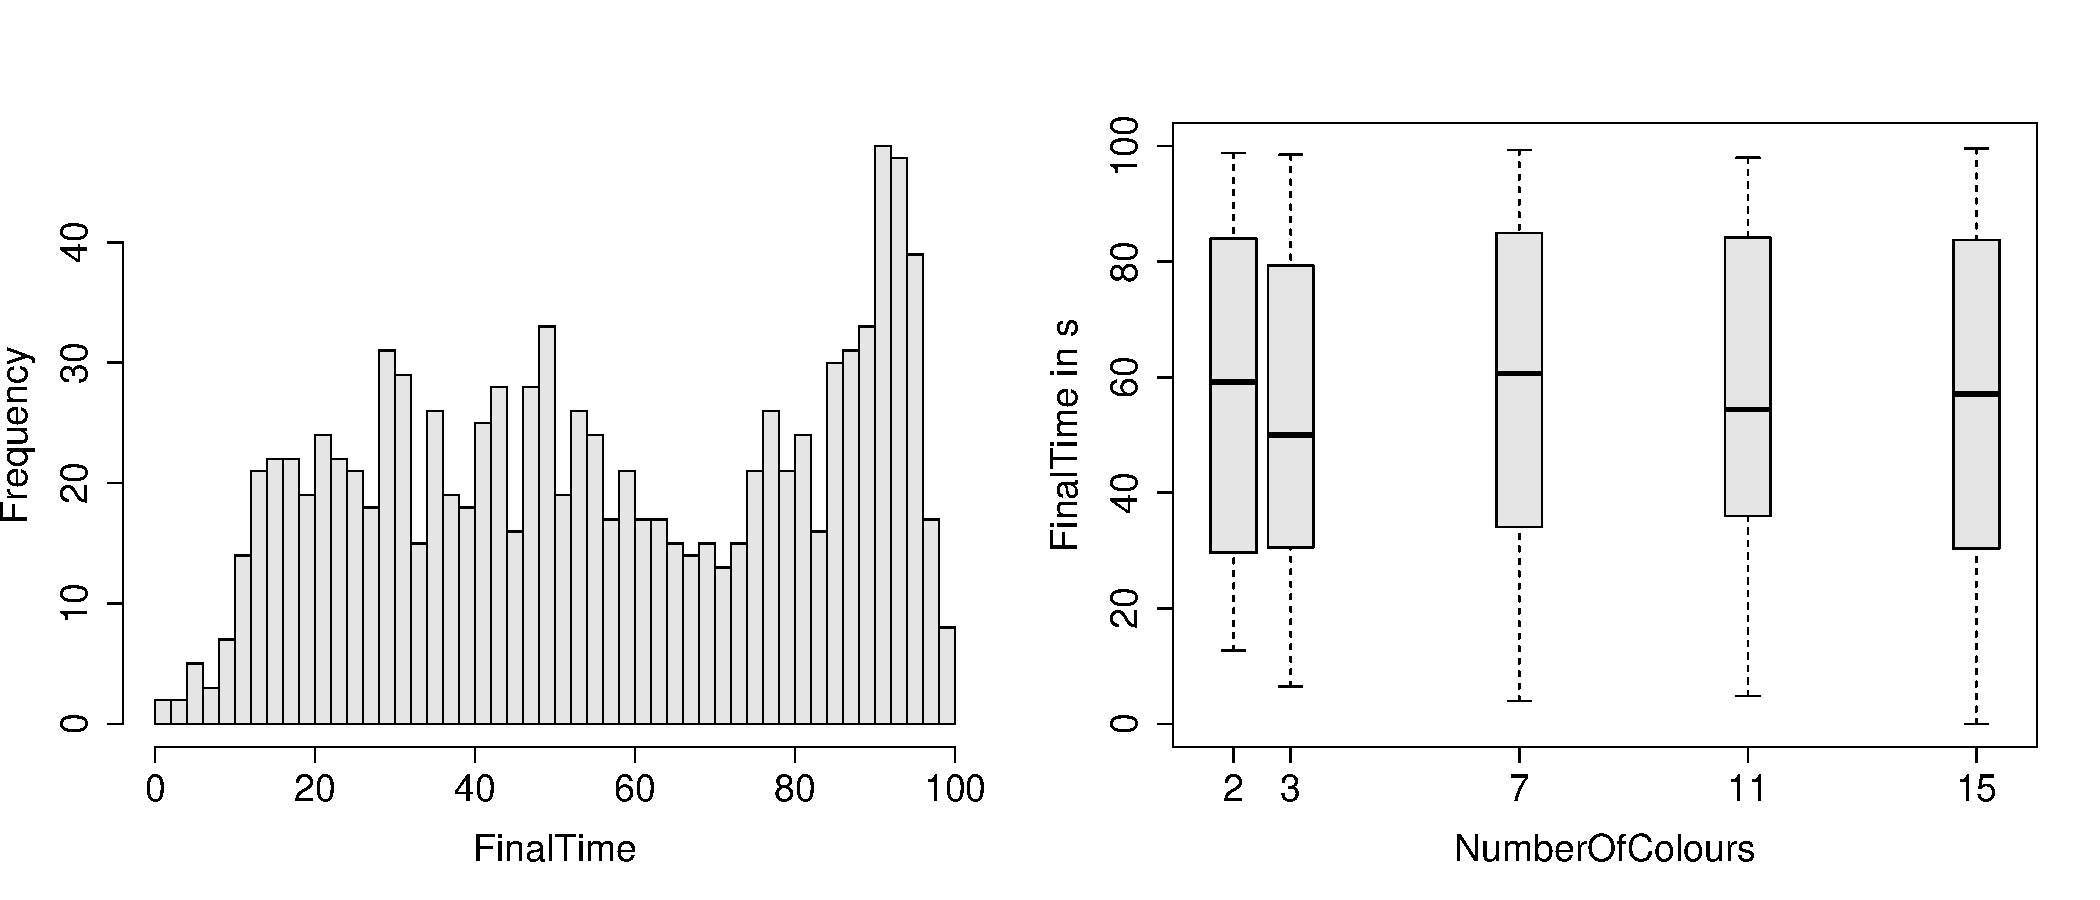
\includegraphics[width = 1\textwidth]{DescriptivesFinalTime.pdf}
\end{center}
\end{figure}
The box plot of \textit{FirstTime} shows similar medians across treatments. The interquartile range is smaller for treatments 2 and 4, and bigger for treatment 3. The standard deviation is the lowest for all time types. The interquartile range is similar among all treatments for the \textit{BestTime}. The values for the medians define a U-shape, with treatment 2 as the apex. The medians for \textit{FinalTime} vary across treatments, yet the interquartile range does not seem to be dependent on the number of colours.

\paragraph{Decision time and number}
The box plots for \textit{DecisionTime} show a wide range, from below 0 seconds to up to 6 seconds for all treatments. The medians are similar and treatment 3 has a wider interquartile range. The majority of participants clicked between 5 and 40 times on boxes per round. The box plot for \textit{DecisionNumber} shows outliers for every treatment, resulting in a range of less than 10 clicks up until 130 clicks per round.
\begin{figure}[htbp] % DistributionDecisionNumber
\begin{center} 
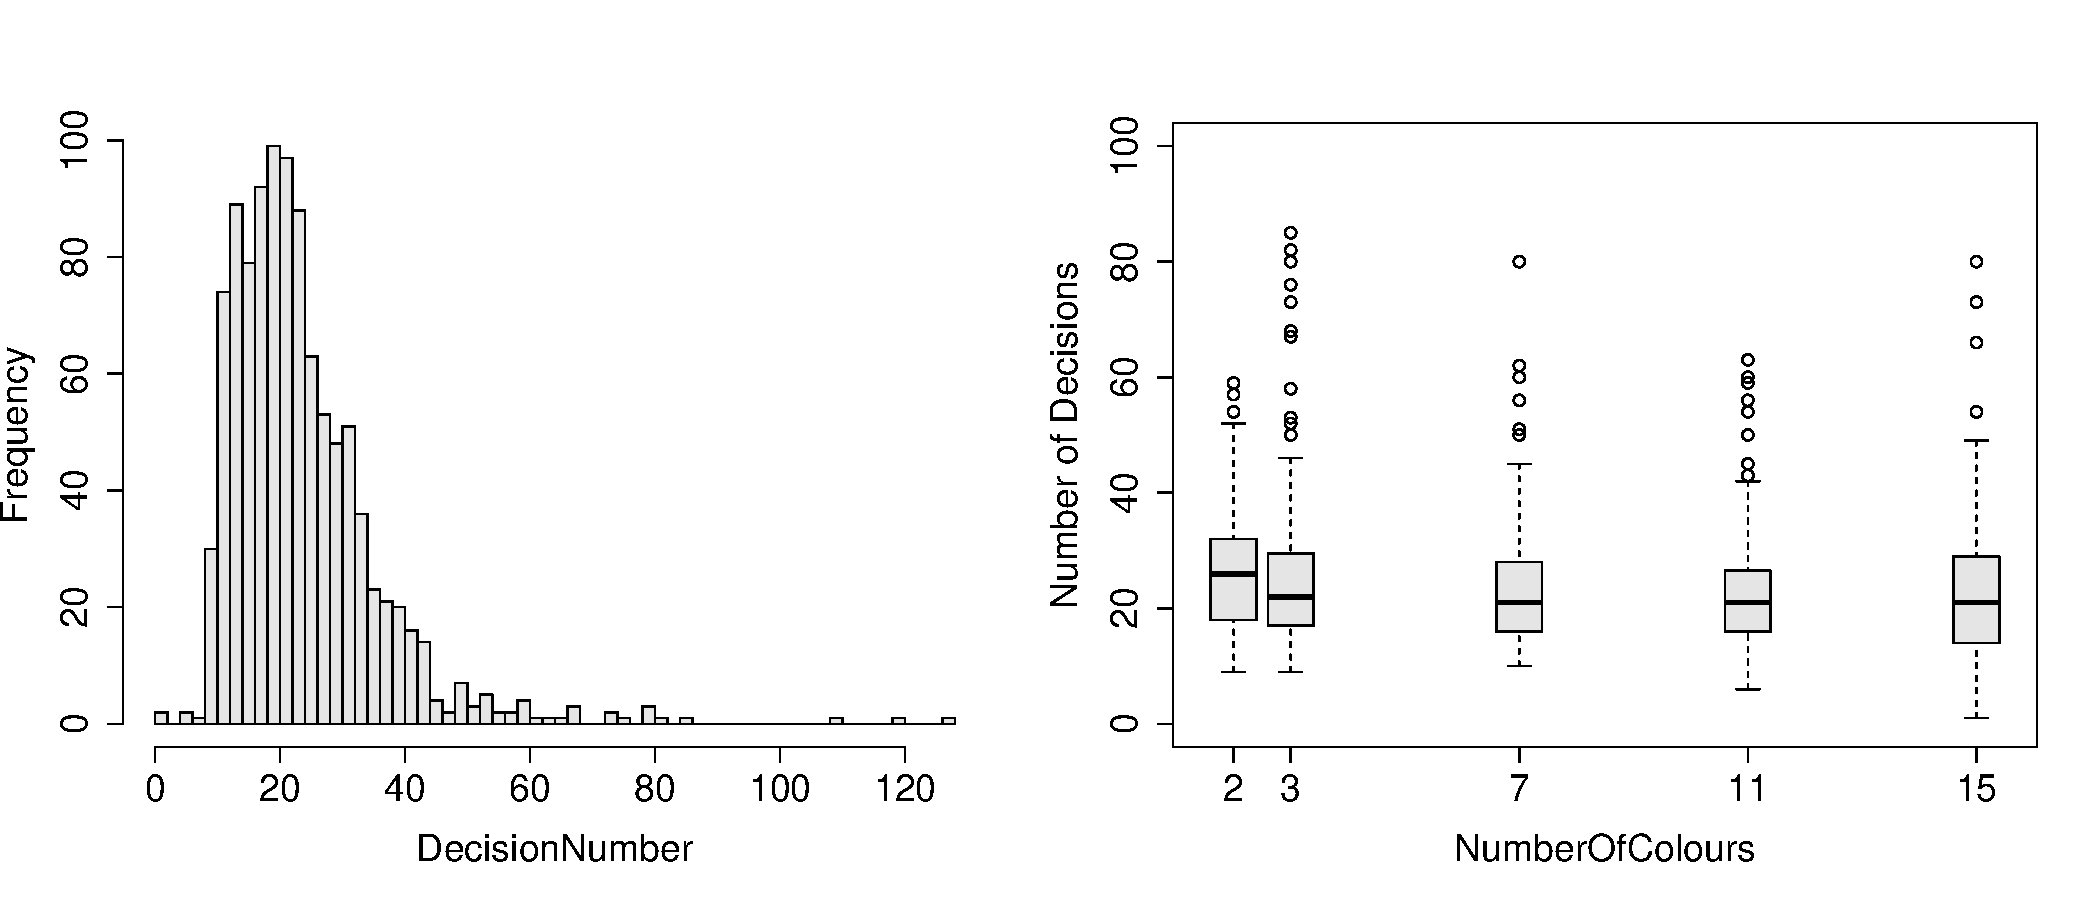
\includegraphics[width = 1\textwidth]{DescriptivesDecisionNumber.pdf}
  \caption{DecisionNumber - Histogram and Box plot}
    \label{DistributionDecisionNumber} 
\end{center}
\end{figure}

%% ===============================
\paragraph{Questionnaire}
\label{ch:Evaluation:sec:DescriptiveStatistics:subsec:Questionnaire}
Figure \ref{ProfilePlot} summarizes each treatment's medians for all the answers. In general, the medians for all treatments show similar values, so the different treatments do not seem to have an influence on the answers.

The mental demand for the task is described as high(5) for all \textit{NumberOfColours} and the pace of the task is defined as medium to rather high. Most of the participants rate their performance as rather successful and define their effort for accomplishing their level of performance as high.
 
There are no significant signs for negative emotions like insecurity or irritation triggered by the experiment, since all treatments indicate a low level of negative emotions. 
Most individuals define "colour" (2) as the main box attribute they are looking at to reach their end result. A high number of individuals take into consideration a combination of the box size and box colour(3) to reach their end result.
The box size (1) is favoured by only a small minority of participants, and other strategies(4) or no strategy(5) have only a minor influence on individuals.
%\begin{landscape}
 \begin{figure}[t] % ProfilePlotAnswer
\begin{center} %ProfilePlotAnswer
\begin{subfigure} 
\centering
 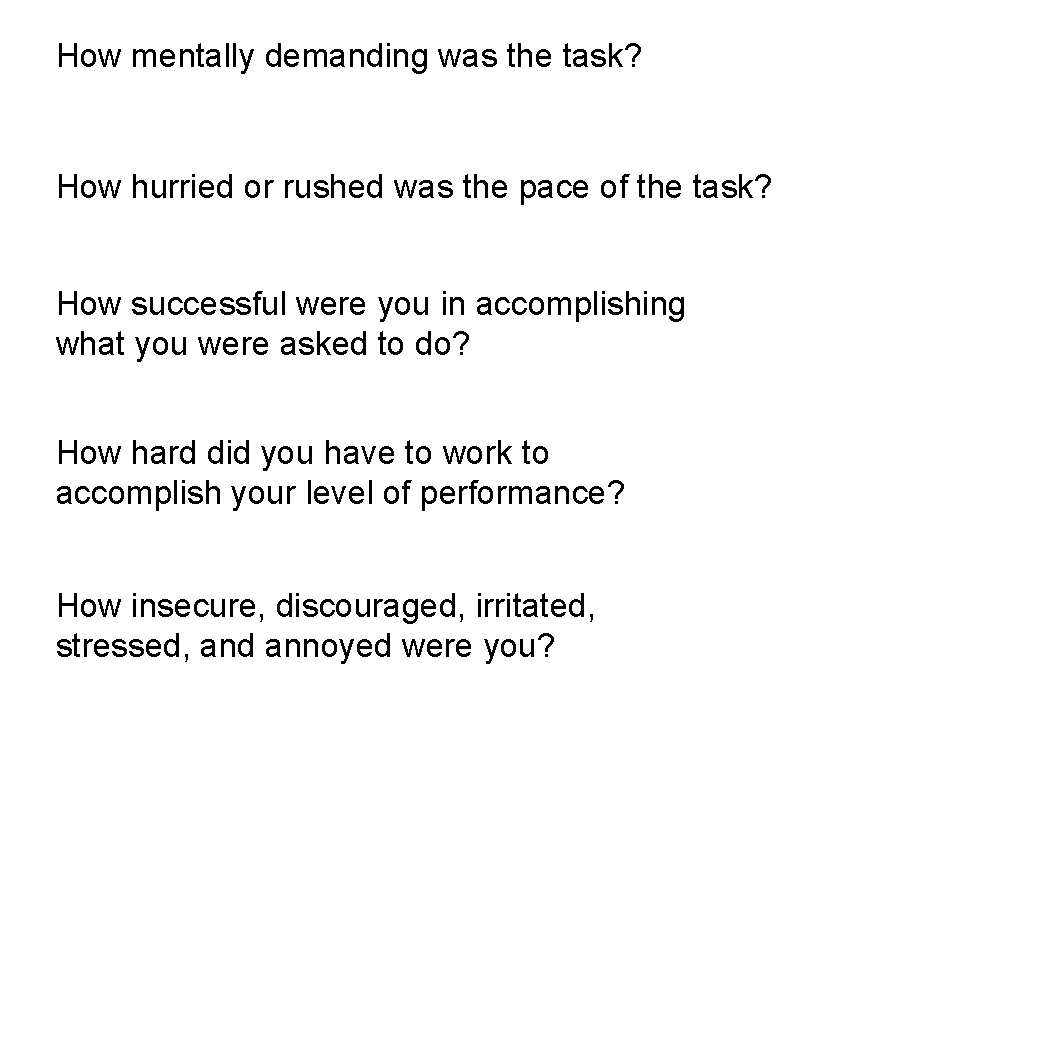
\includegraphics[height = 0.4\textwidth]{ProfilePlotLegend.pdf}
\end{subfigure} 
\begin{subfigure}
\centering
 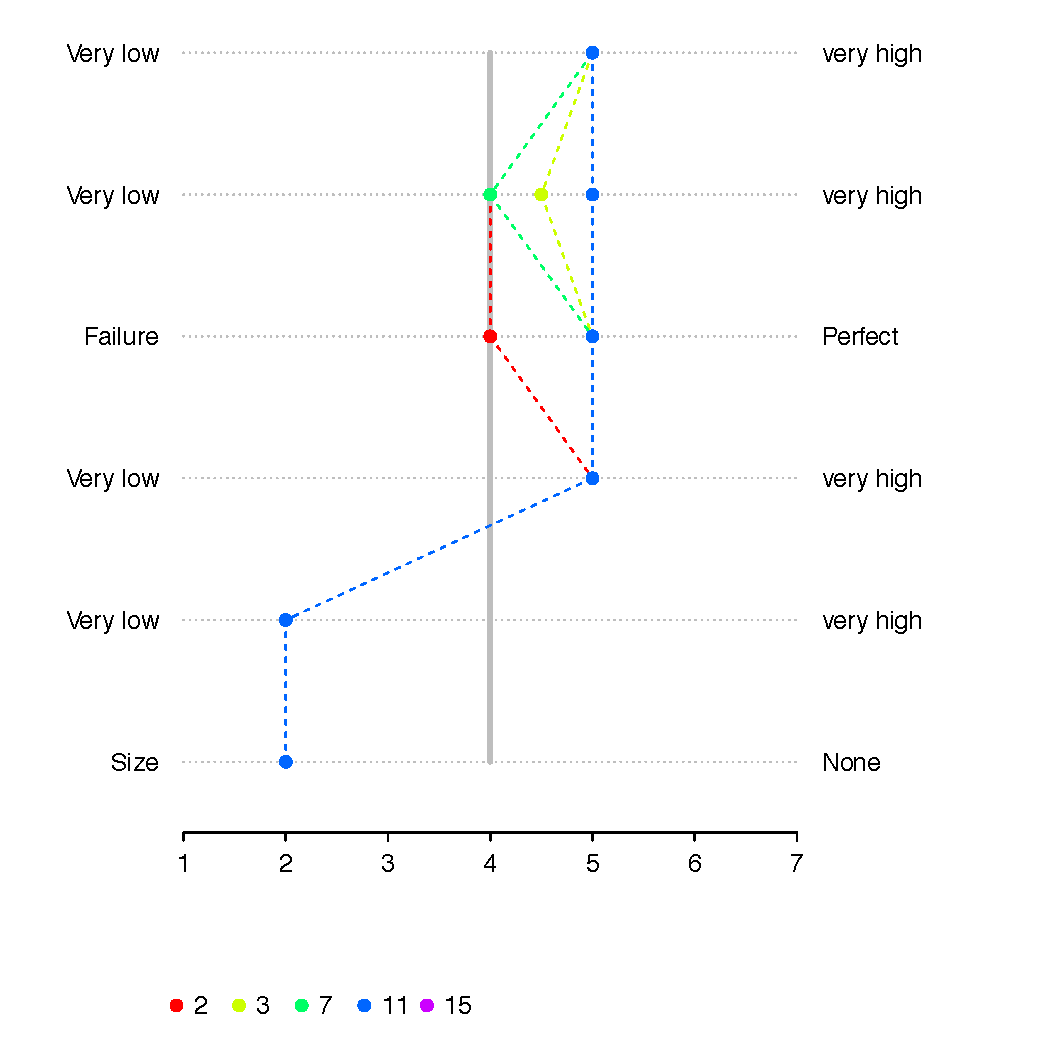
\includegraphics[height = 0.4\textwidth]{ProfilePlotAnswer.pdf}
\end{subfigure}
\begin{subfigure} 
 \raggedright
 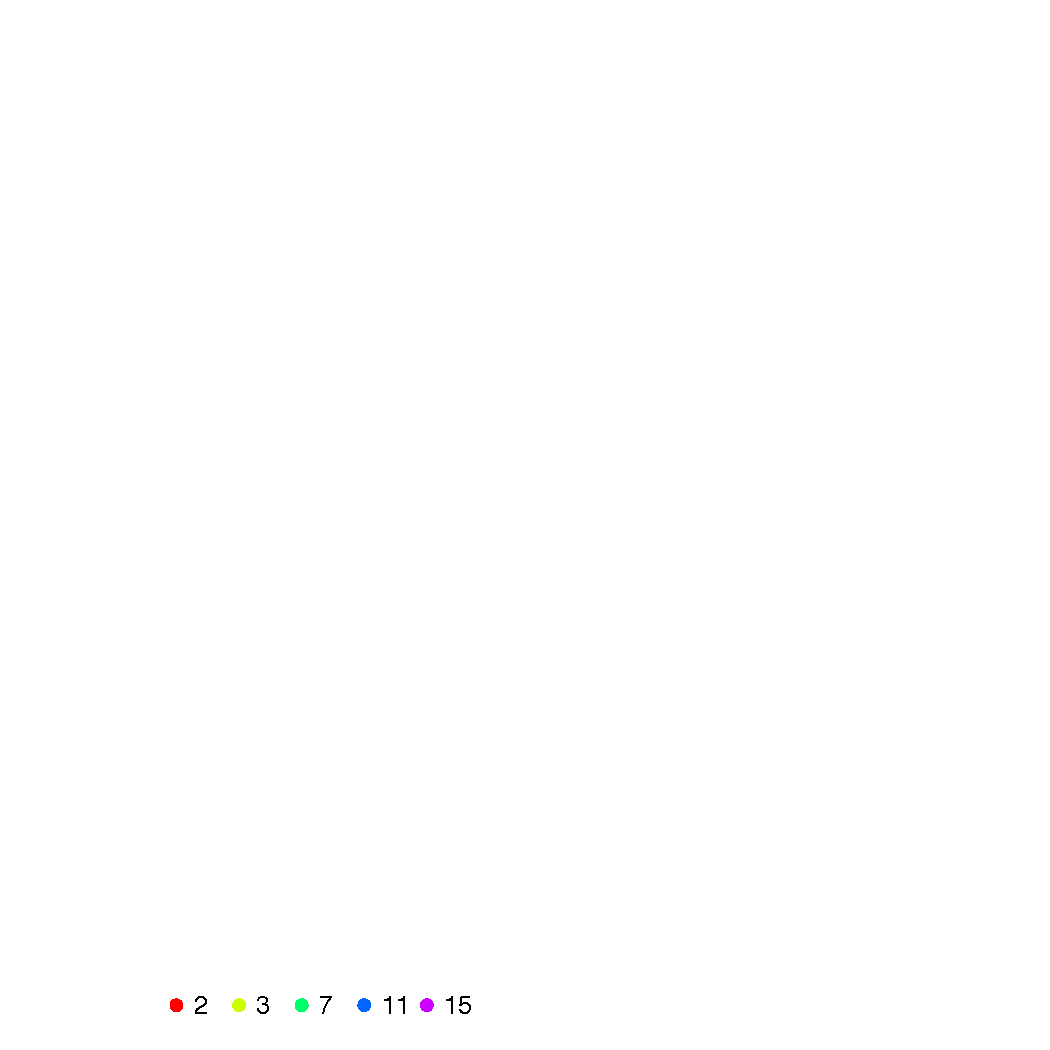
\includegraphics[height = 0.07\textwidth]{ProfilePlotLegend2.pdf}
\end{subfigure}    
  \caption{Profile Plot}
  \label{ProfilePlot}
\end{center}
\end{figure}
%\end{landscape}

\begin{figure}[htbp] % Question6	
\begin{center} 
\begin{subfigure} 
\centering
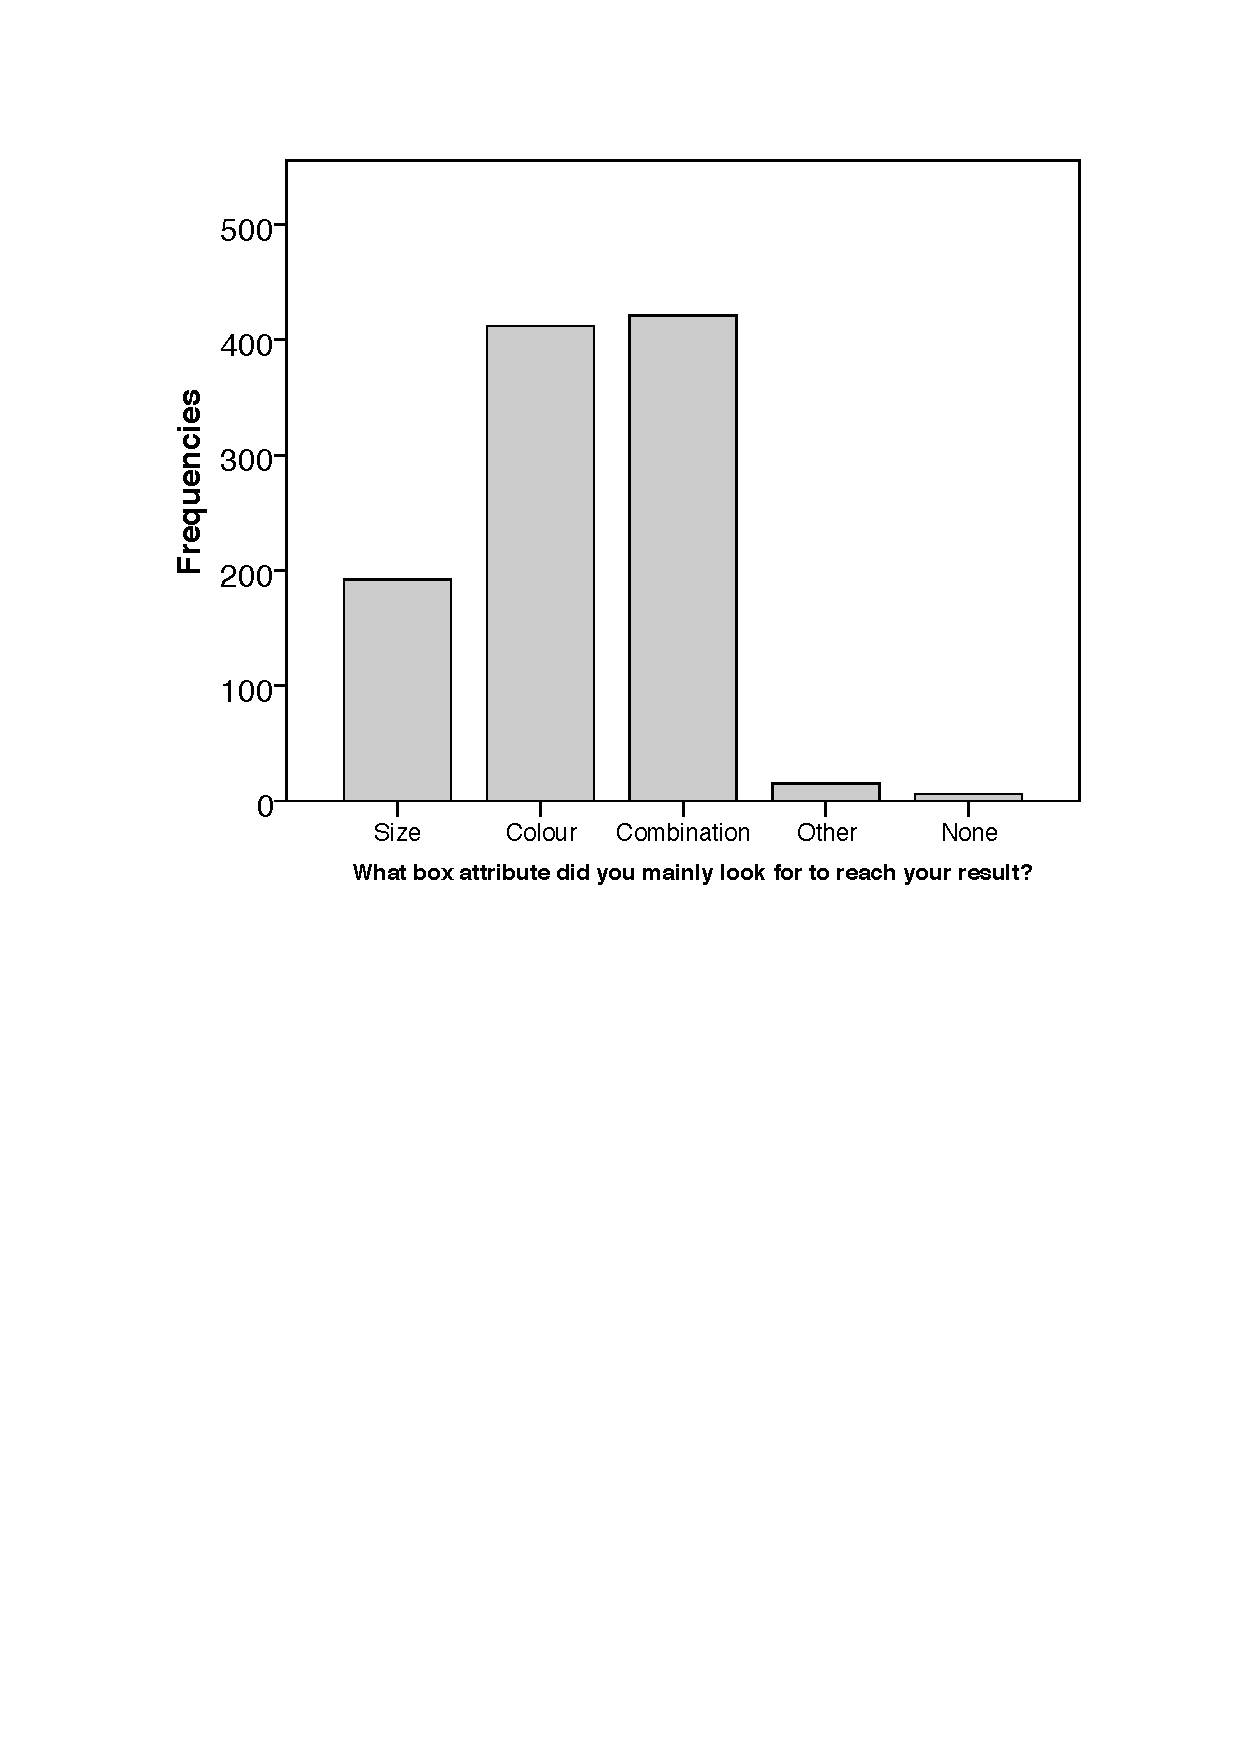
\includegraphics[height = 0.38\textwidth]{HistogramQuestion6.pdf}
\end{subfigure} 
\begin{subfigure} 
\centering
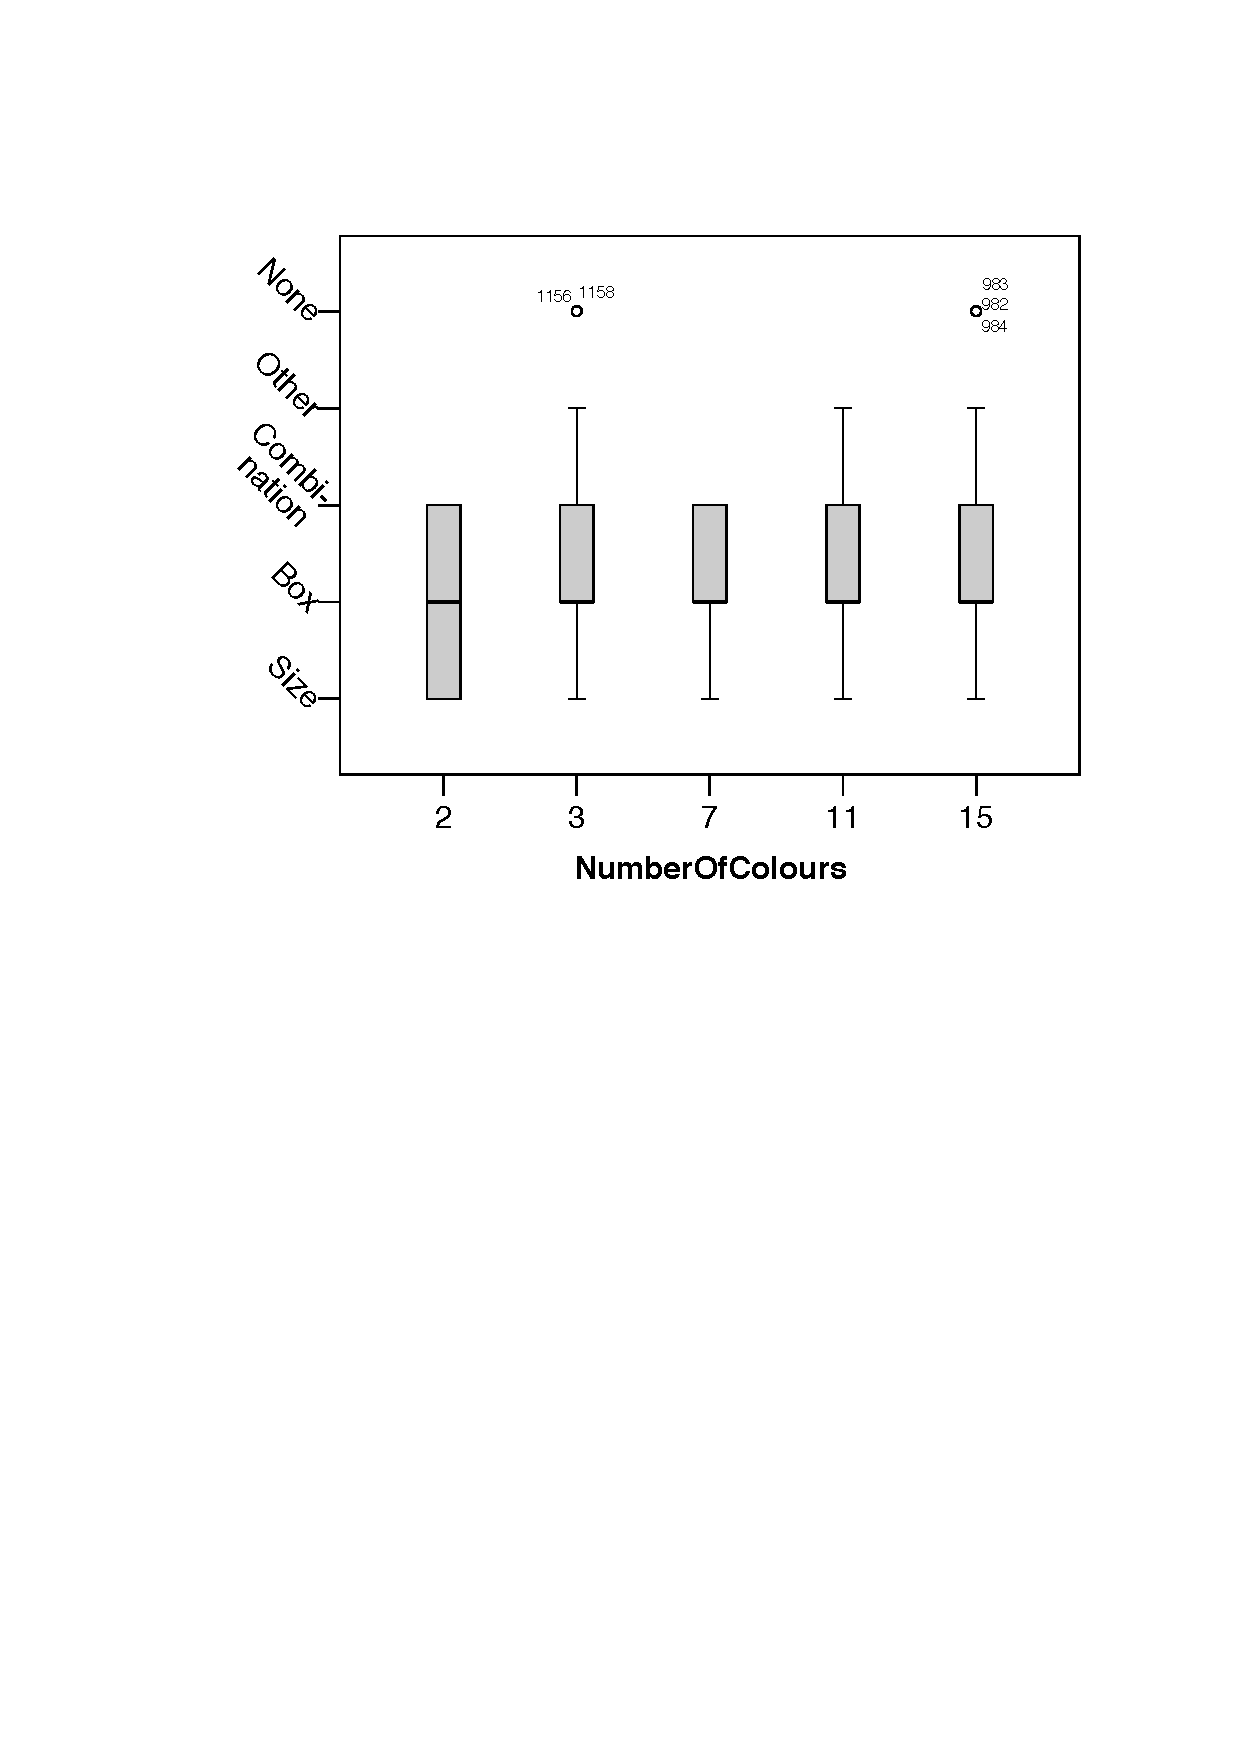
\includegraphics[height = 0.38\textwidth]{BoxplotQuestion6.pdf}
\end{subfigure}
  \caption[Question 6 - Histogram and Box plot]{Question 6 - Size (1), Colour (2), Combination (3), Other (4), None (5)}
    \label{Question6} 
\end{center}
\end{figure} 
\newpage
% ===============================
\paragraph{Correlation of variables}
Figure \ref{Correlation} illustrates the correlation between all the variables. The bigger the size of the circles, the greater the magnitude of the correlation. The green colour represents a positive correlation and the red colour represents a negative linear correlation, so big green circles refer to a high positive linear correlation.\\
The two main correlation groups can be identified as the different result and time types since they both show a high correlation. The correlation between these two groups is smaller than within the groups, but is still positive. This result indicates that the more time a participant takes for completing the round, the more successful he or she will be, and vice versa.

The linear correlation between the time and result variables, and the independent variables \textit{Round} and \textit{NumberOfColours}, is only small, yet the \textit{DecisionTime} shows a higher positive correlation for the \textit{NumberOfColours} and a more negative correlation for \textit{Round}. In other words, the more colours that are added to the game, the more time it takes the participant, on average, to make a decision, and the decision time decreases over the rounds played.

The \textit{DecisionNumber} is positively correlated to the result and time variables, showing the highest correlation value for \textit{FinalTime} and \textit{BestTime}. The correlation between the mental demand of the task (Question 1) and the level of how hard participants work to accomplish the task (Question 4) is the highest for all answers' correlations, even though it indicates only a medium correlation. Smaller but still positive correlations with the mental demand, can be identified for the pace of the task (Question 2) and the level of negative emotions (Question 5).

A small negative correlation is detectable for Question 1, Question 4 and Question 5, as well as the performance variables. Therefore, participants with a higher result indicate a lower mental demand, a lower level of effort and a lower level of negative emotions. Interestingly, the correlation matrix does not show a high correlation between how successful the participants are and how successful they feel (Question 2). 
 \begin{figure}[h] % 130315_CorrelationAction
\begin{center} %130315_CorrelationAction
  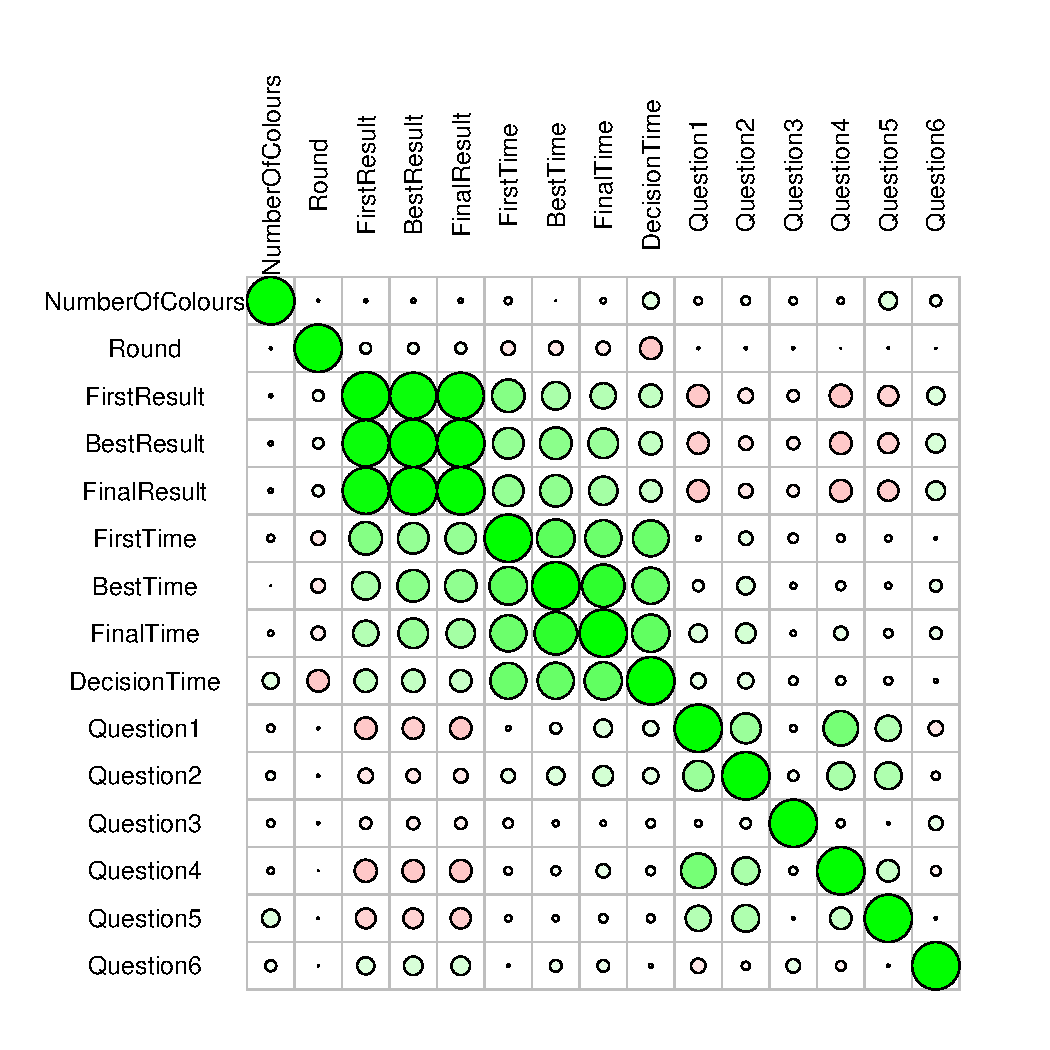
\includegraphics[height = 1\textwidth]{CorrelationAction.pdf}
  \caption{Correlation of variables}
  \label{Correlation}
\end{center}
\end{figure}
